\newpage
\subsection{Test di Unità}
Questa tipologia di test è molto utile per veirificare il funzionamento delle singole unità che compongono MaaS.
Verrà utilizzata la seguente notazione:
	\begin{center}
		TU-\textit{IDComponente}
	\end{center}
dove \textit{IdComponente} corrisponde al codice identificativo (crescente) del componente preso in esame dal test.

\begin{center}
  
  \begin{table}[H]
    \centering
    \begin{tabular}{ | >{\centering}p{3cm} | >{\centering}p{6cm} | >{\centering}p{1.5cm} | >{\centering}p{2cm} | }
      \textbf{Test Sistema} & \textbf{Descrizione} & \textbf{Stato} & \textbf{Requisito} \tabularnewline \hline
      
      % example & bla & blabla & blablabla \tabularnewline \hline

\section{Backend}
\subsection{Formalismo utilizzato}
L'utilizzo del framework ExpressJS come base per il server ha evidenziato la necessità di regolamentare alcune convenzioni utilizzate. Queste convenzioni riguardano il formalismo utilizzato per la rappresentazione in quanto concetti come moduli, middlewares e first-class function non hanno una corrispondenza diretta nei diagrammi UML.
%I moduli verranno rappresentati come classi.

%% DA FINIRE E DEFINIRE CON MATTEO

\subsection{Descrizione generale}
L'implementazione scelta per il backend dell'applicazione è un server con architettura REST. Ciò implica che:
\begin{itemize}
\item l'applicazione renda disponibili le sue funzioni in veste di risorse web;
\item ogni risorsa resa disponibile è indirizzabile univocamente utilizzando un indirizzo URL;
\item l'interfaccia delle risorse deve essere uniforme e deve garantire un insieme ben definito di operazioni e una gestione priva di stato delle operazioni.
\end{itemize}

Tale architettura permette l'indipendenza completa tra backend e frontend, permettendo così a espansioni su altre piattaforme senza dover modificare il backend dell'applicazione.

L'architettura del backend segue il design patter MVC (\textbf{M}odel \textbf{V}iew \textbf{C}ontroller) per quanto concerne i ruoli di Model e Controller. 
Il ruolo di Controller tuttavia, non essendo implementato nativamente in Express, verrà implementato da uno stack di middleware come suggerito dal framework.
La parte View, invece, è rapprestata dal frontend, costituito da componenti definiti con React e disposti secondo l'architettura Flux.

\subsection{Descrizione dei package}
Il seguente diagramma mostra l'architettura generale del backend.
\begin{figure}[H]
\centering
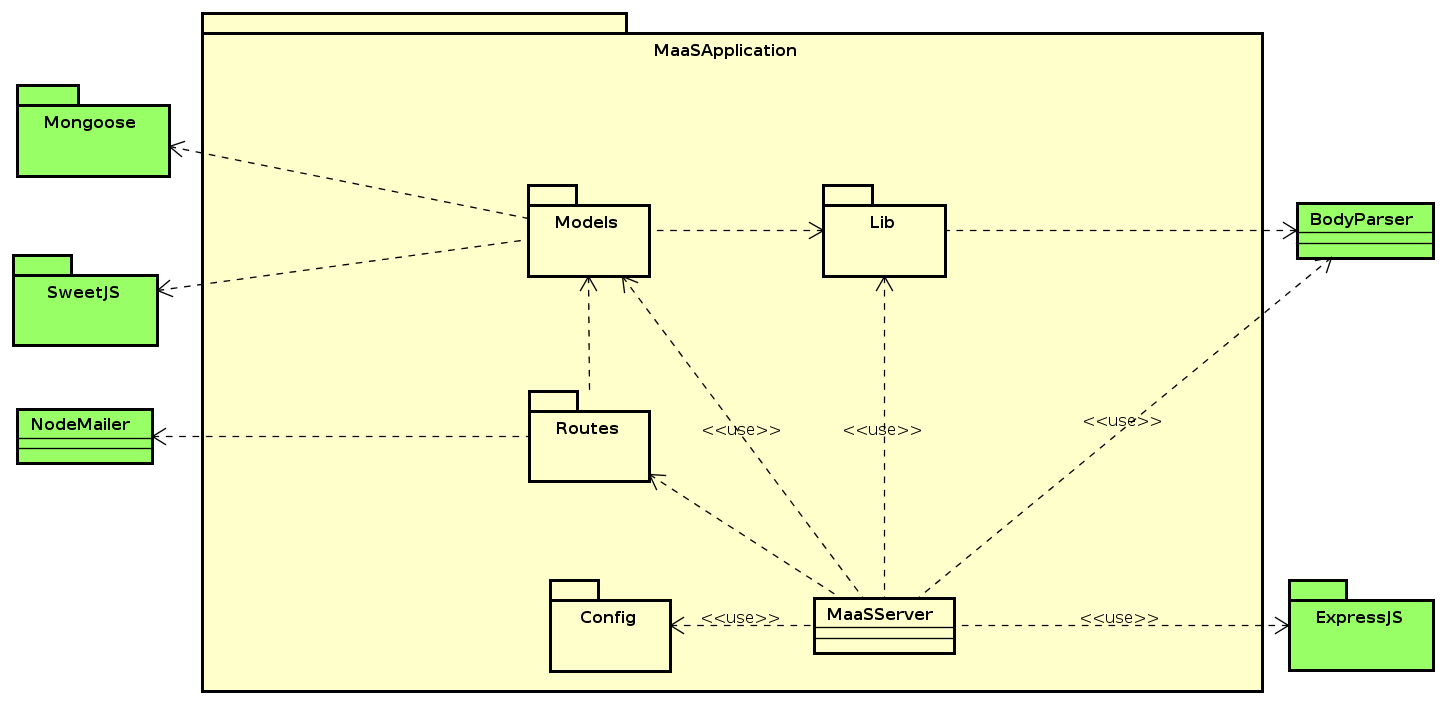
\includegraphics[width=0.8\textwidth]{res/sections/backend/generale.png}
\caption{Diagramma dei package}
\end{figure}

\subsubsection{Package MaaSApplication}
\paragraph*{Descrizione}
Package che racchiude tutta l'applicazione MaaS.

\paragraph*{Package contenuti}
\begin{itemize}
\item Models
\item Routes
\item Config
\item Lib
\end{itemize}

\paragraph*{Moduli contenuti}
\begin{itemize}
\item MaaSServer
\end{itemize}

\begin{figure}[H]
\centering
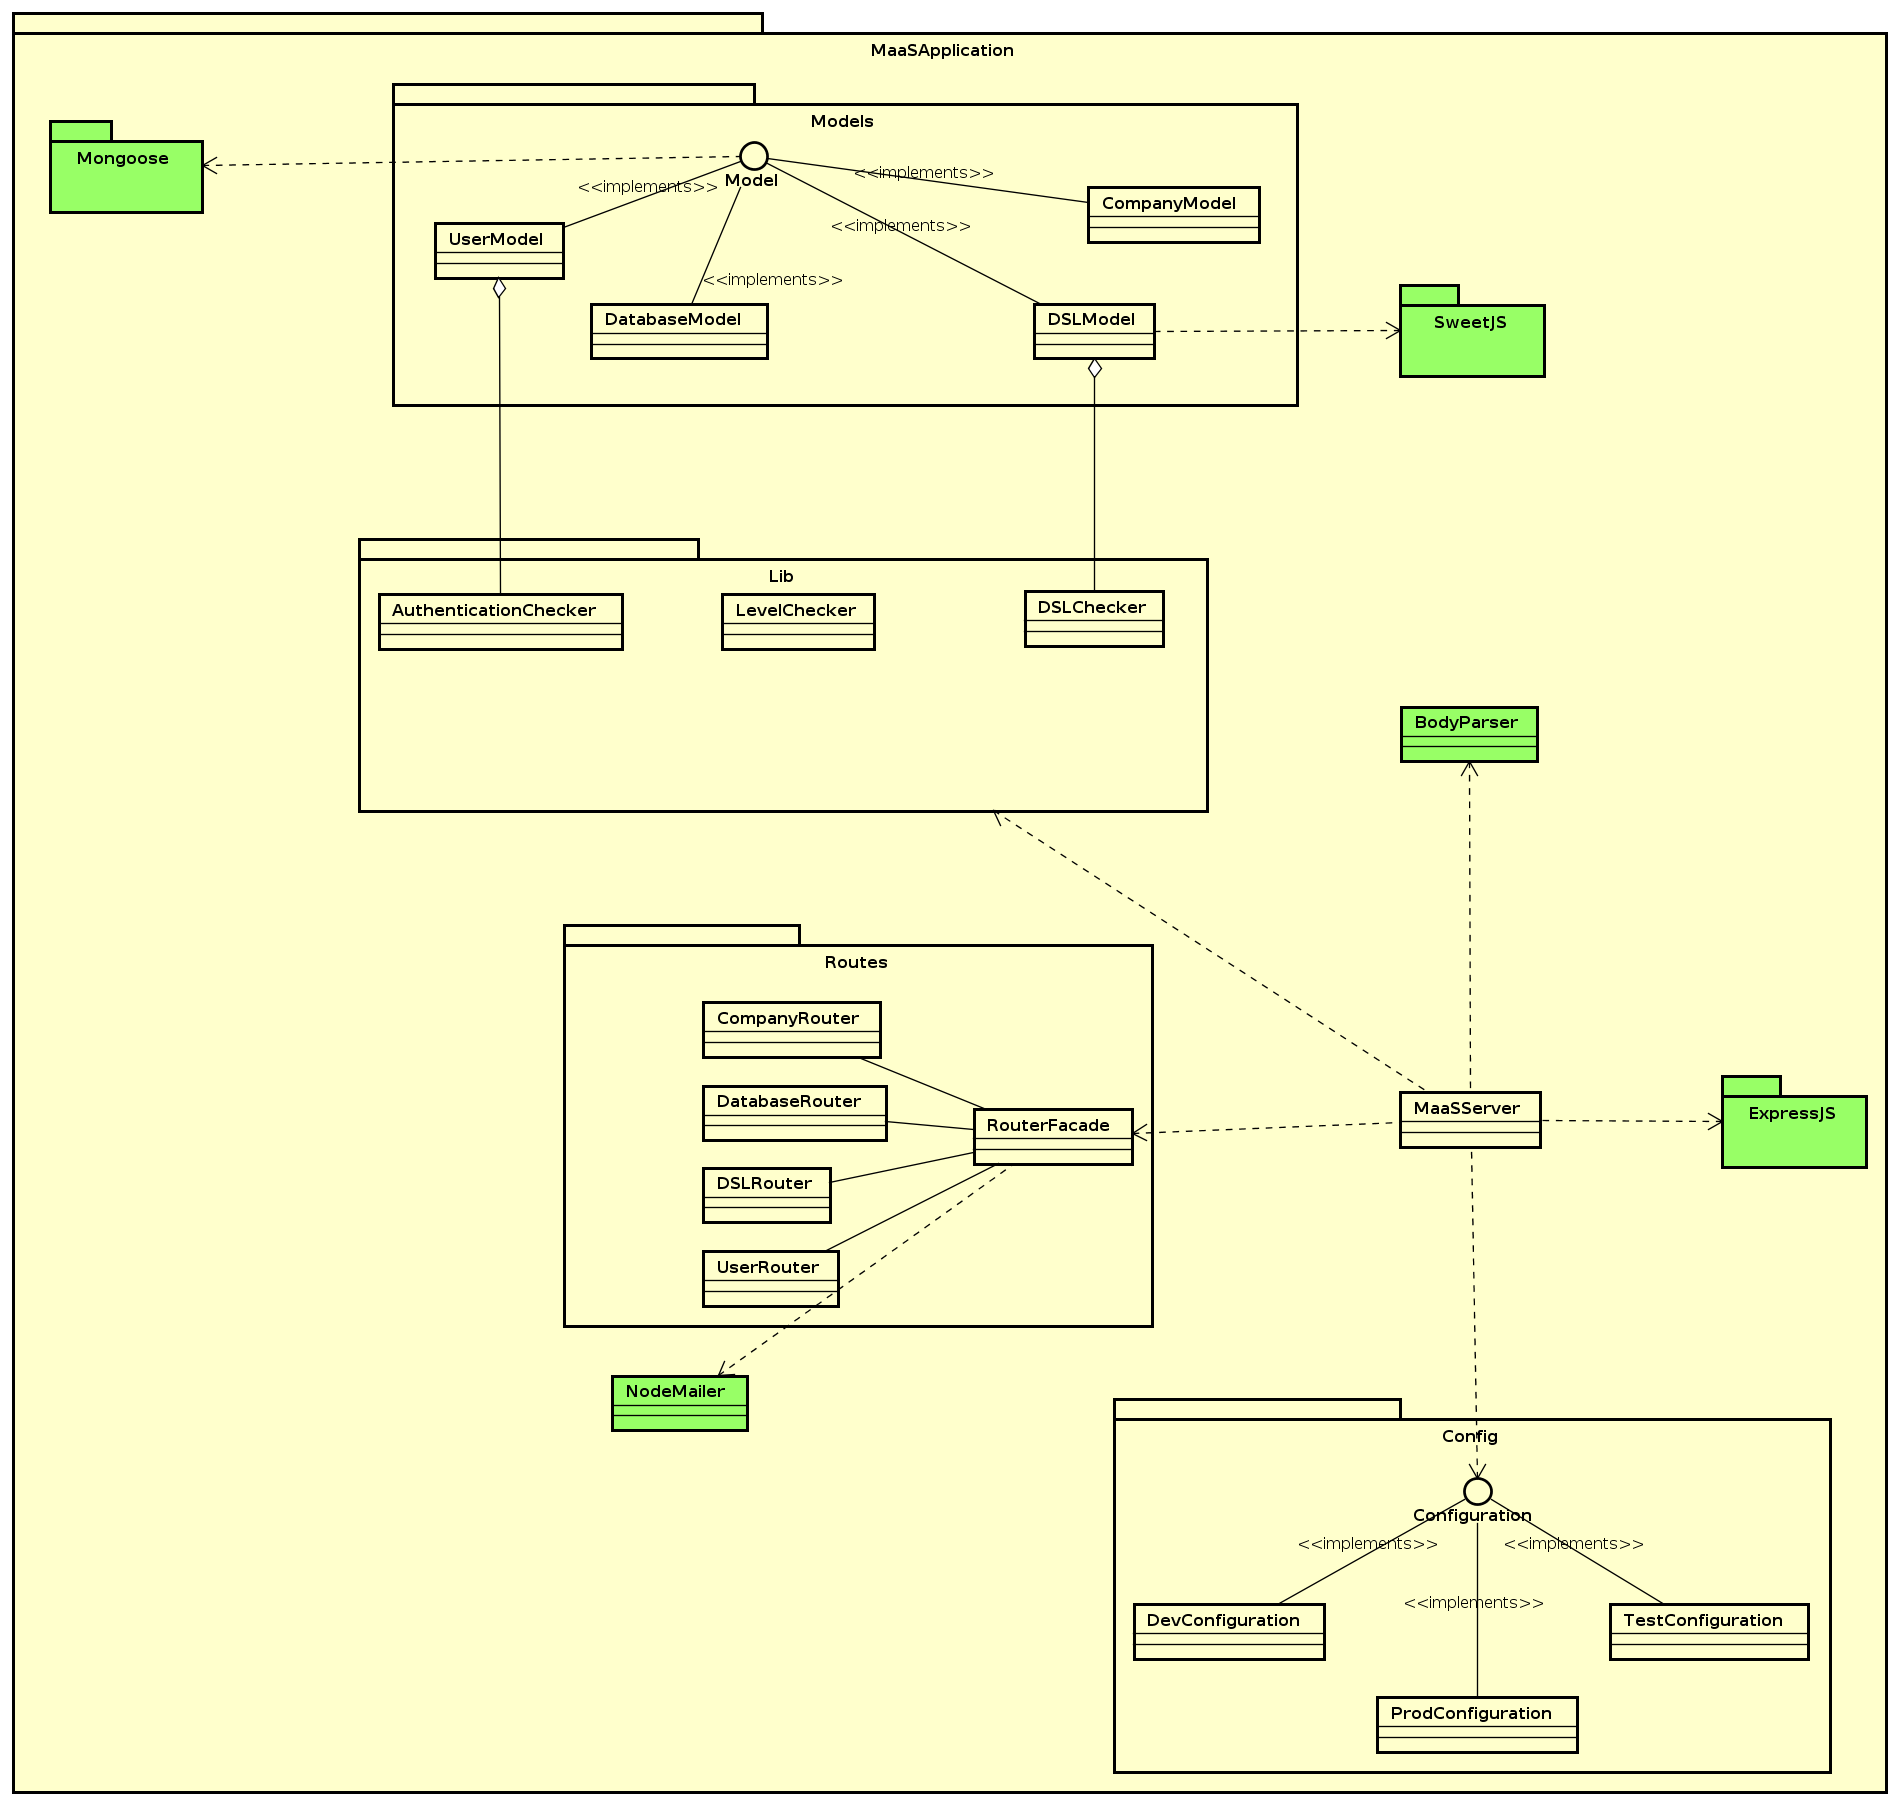
\includegraphics[width=0.8\textwidth]{res/sections/backend/collegamenti.png}
\caption{Diagramma dei package completo dei componenti per ciascun package}
\end{figure}

\subsection{Package Models}
\paragraph*{Descrizione}
Package che racchiude i moduli contenenti la business logic dell'applicazione. Ciascuno di questi moduli implementa un modello Mongoose e definisce i metodi con cui interagirvi (aggiungere, rimuovere e modificare i contenuti). \\
Rappresenta la parte M (Model) del design pattern MVC.

\paragraph*{Moduli contenuti}
\begin{itemize}
\item UserModel
\item DSLModel
\item CompanyModel
\item DatabaseModel
\end{itemize}

\paragraph*{Interfacce contenute}
\begin{itemize}
\item Model
\end{itemize}

\begin{figure}[H]
\centering
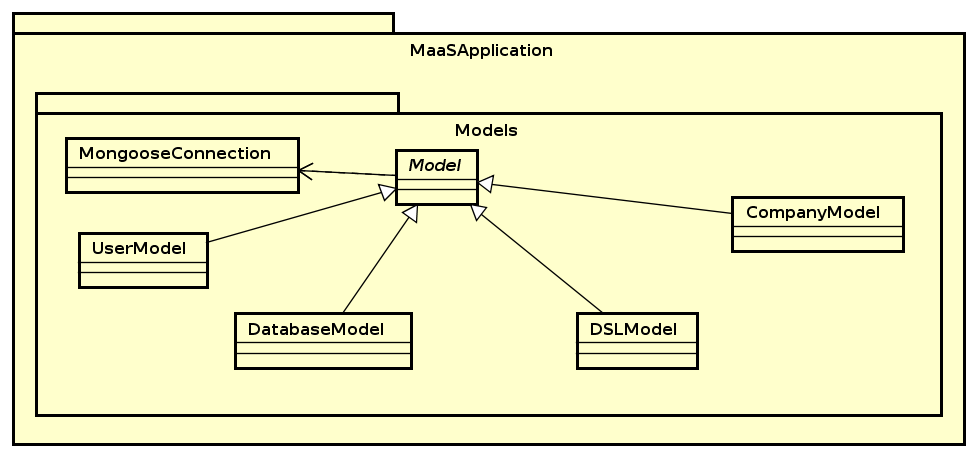
\includegraphics[width=0.8\textwidth]{res/sections/backend/models.png}
\caption{Diagramma delle classi del package Models}
\end{figure}

\subsubsection{UserModel}
\paragraph*{Descrizione}

Racchiude la business logic legata agli utenti. Viene implementato tramite Module pattern di Javascript. 

\paragraph*{Utilizzo}
Il modello viene utilizzato sia per la rappresentazione di un utente nell'applicazione, sia per l'autenticazione nel sistema.

\paragraph*{Relazioni con altri moduli}
\begin{itemize}
\item Mongoose
\item Mongoose-validator
\item Lib::AuthenticationChecker
\end{itemize}

\subsubsection{CompanyModel}
\paragraph*{Descrizione}
Racchiude la business logic legata alle Company. Viene implementato tramite Module pattern di Javascript. 

\paragraph*{Utilizzo}
Il modello rappresenta una Company nel sistema.

\paragraph*{Relazioni con altri moduli}
\begin{itemize}
\item Mongoose
\item Mongoose-validator
\end{itemize}

\paragraph{DatabaseModel}
\paragraph*{Descrizione}

Racchiude la business logic legata al collegamento con i database delle Company. Viene implementato tramite Module pattern di Javascript. 

\paragraph*{Utilizzo}
Il modello rappresenta la connessione ad un database aziendale di una company. Contiene i dati per effettuare l'accesso al database e il riferimento alle collections definite su tale database, permettendo così all'utente di poter definire per ciascuna collection la possibilità di interagirvi da parte di tutti i membri della propria Company o solo degli admin.

\paragraph*{Relazioni con altri moduli}
\begin{itemize}
\item Mongoose
\item Mongoose-validator
\end{itemize}

\paragraph{DSLModel}
\paragraph*{Descrizione}

Racchiude la business logic legata alle specifiche DSL. Viene implementato tramite Module pattern di Javascript. 

\paragraph*{Utilizzo}
Il modello viene utilizzato per la rappresentazione delle specifiche DSL. Contiene i dati di tali specifiche e le funzioni per poter estrarre i dati richiesti da una specifica DSL.

\paragraph*{Relazioni con altri moduli}
\begin{itemize}
\item Mongoose
\item Mongoose-validator
\item DSLChecker
\item DatabaseModel
\end{itemize}

\paragraph{Model}
\paragraph*{Descrizione}
Interfaccia comune a tutti i modelli usati da MaaS.

\paragraph*{Utilizzo}
Viene utilizzata come base per UserModel, CompanyModel, DSLModel e DatabaseModel.

\paragraph*{Relazione con altri moduli}
\begin{itemize}
\item Mongoose
\item UserModel
\item CompanyModel
\item DSLModel
\item DatabaseModel
\end{itemize}

\subsubsection{Package Routes}
\paragraph*{Descrizione}
Il package Routes contiene l'implementazione dei Router definiti da ExpressJS. Il package è costituito da una serie di moduli che implementano gli endpoint per le API.
I moduli vengono suddivisi in base al modello che utilizzano. Ciascuna route definita inoltre ha il compito di richiamare i middleware necessari.
La definizione delle API seguirà la descrizione riportata nella sezione apposita di questo documento.\\
Reppresenta la parte C (Controller) del design pattern MVC.

\paragraph*{Moduli contenuti}
\begin{itemize}
\item UserRouter
\item CompanyRouter
\item DSLRouter
\item DatabaseRouter
\item RouterFacade
\end{itemize}

\paragraph*{Interfacce contenute}
\begin{itemize}
\item Router
\end{itemize}

\begin{figure}[H]
\centering
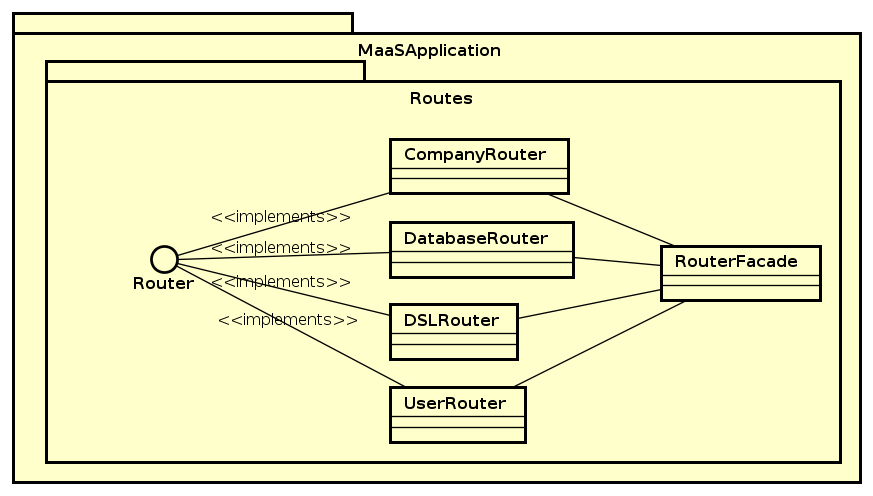
\includegraphics[width=0.8\textwidth]{res/sections/backend/routes.png}
\caption{Diagramma delle classi del package Routes}
\end{figure}

\paragraph{UserRouter}
\paragraph*{Descrizione}
Questo modulo contiene la definizione degli endpoint riguardanti gli utenti. 

\paragraph*{Relazione con altri moduli}
\begin{itemize}
\item AuthenticationChecker
\item UserModel
\end{itemize}

\paragraph{CompanyRouter}
\paragraph*{Descrizione}
Questo modulo contiene la definizione degli endpoint riguardanti le company.

\paragraph*{Relazione con altri moduli}
\begin{itemize}
\item AuthenticationChecker
\item CompanyModel
\end{itemize}

\paragraph{DSLRouter}
\paragraph*{Descrizione}
Questo modulo contiene la definizione degli endpoint riguardanti le specifiche DSL.

\paragraph*{Relazione con altri moduli}
\begin{itemize}
\item AuthenticationChecker
\item DSLModel
\end{itemize}

\paragraph{DatabaseRouter}
\paragraph*{Descrizione}
Questo modulo contiene la definizione degli endpoint riguardanti le connessioni ai database aziendali.

\paragraph*{Relazione con altri moduli}
\begin{itemize}
\item AuthenticationChecker
\item DatabaseModel
\end{itemize}

\paragraph{RouterFacade}
\paragraph*{Descrizione}
Oggetto che implementa il Facade Design Pattern. Tale oggetto incorpora tutti gli endpoint definiti dagli altri router.

\paragraph*{Relazione con altri moduli}
\begin{itemize}
\item AuthenticationChecker
\item UserRouter
\item CompanyRouter
\item DSLRouter
\item DatabaseRouter
\end{itemize}

\paragraph{Router}
\paragraph*{Descrizione}
Interfaccia comune ai router usati da MaaS.

\paragraph*{Utilizzo}
Viene utilizzata come base per UserRouter, CompanyRouter, DSLRouter e DatabaseRouter.

\paragraph*{Relazione con altri moduli}
\begin{itemize}
\item BodyParser
\item UserRouter
\item CompanyRouter
\item DSLRouter
\item DatabaseRouter
\end{itemize}

\subsubsection{Package Config}
\paragraph*{Descrizione}
Questo package contiene la classe Configuration che, in base alla variabile d'ambiente NODE\_ENV, restituisce l'oggetto contenente tutte le informazioni utili alla configurazione del server.

\paragraph*{Moduli contenuti}
\begin{itemize}
\item Configuration
\item DevConfiguration
\item TestConfiguration
\item ProdConfiguration
\end{itemize}

\paragraph*{Interfacce contenute}
\begin{itemize}
\item Configuration
\end{itemize}

\begin{figure}[H]
\centering
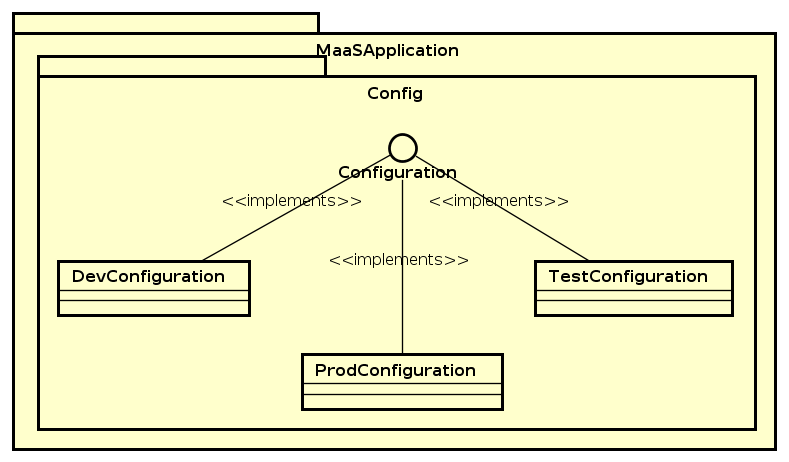
\includegraphics[width=0.8\textwidth]{res/sections/backend/config.png}
\caption{Diagramma delle classi del package Config}
\end{figure}

\paragraph{DevConfiguration}
\paragraph*{Descrizione}
Configurazione usata durante lo sviluppo.

\paragraph*{Utilizzo}
Viene utilizzata per configurare l'ambiente di lavoro durante lo sviluppo di MaaS.

\paragraph{TestConfiguration}
\paragraph*{Descrizione}
Configurazione usata durante il test.

\paragraph*{Utilizzo}
Viene utilizzata per configurare l'ambiente di lavoro durante il test di MaaS.

\paragraph{ProdConfiguration}
\paragraph*{Descrizione}
Configurazione usata per il rilascio.

\paragraph*{Utilizzo}
Viene utilizzata per configurare l'ambiente di lavoro per la consegna di MaaS.

\paragraph{Configuration}
\paragraph*{Descrizione}
Interfaccia comune alle configurazioni usate da MaaS.

\paragraph*{Utilizzo}
Viene utilizzata come base per DevConfiguration, TestConfiguration e ProdConfiguration.

\paragraph*{Relazione con altri moduli}
\begin{itemize}
\item MaaSServer
\end{itemize}

\subsubsection{Package Lib}
\paragraph*{Descrizione}
Questo package contiene tutti i moduli di supporto al sistema e i middlewares generici per ExpressJS.

\paragraph*{Moduli contenuti}
\begin{itemize}
\item LevelChecker
\item AuthenticationChecker
\item DSLChecker
\end{itemize}

\paragraph{Interfacce contenute}
\begin{itemize}
\item Middleware
\end{itemize}

\begin{figure}[H]
\centering
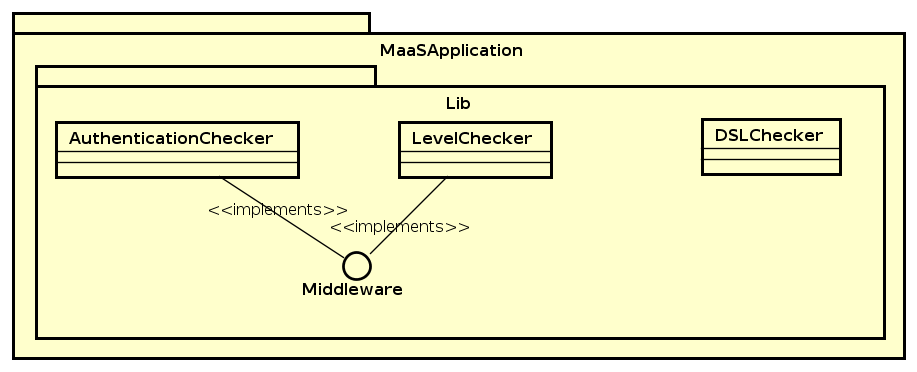
\includegraphics[width=0.8\textwidth]{res/sections/backend/lib.png}
\caption{Diagramma delle classi del package Lib}
\end{figure}

\paragraph{LevelChecker}
\paragraph*{Descrizione}
Middleware che si occupa di verificare se l'utente che effettua una richiesta al server ha i livelli minimi di accesso per poterla eseguire.

\paragraph*{Utilizzo}
Viene utilizzato nelle routes in cui deve essere garantito un livello utente minimo di accesso per portare a termine la richiesta.

\paragraph*{Relazione con altri moduli}
\begin{itemize}
\item Router
\end{itemize}

\paragraph{AuthenticationChecker}
\paragraph*{Descrizione}
Modulo che definisce due middleware: uno per effettuare il login, l'altro per l'autenticazione di una richiesta.

\paragraph*{Utilizzo}
Questo modulo viene utilizzato per definire l'endpoint per effettuare il login all'applicazione e offre il middleware che permette di autenticare le richieste. Tale middleware si occuperà di estrarre il token dalle richieste, verificarne la correttezza e aggiungere l'utente verificato nella richiesta per i prossimi middleware.

\paragraph*{Relazione con altri moduli}
\begin{itemize}
\item Router
\end{itemize}

\paragraph{DSLChecker}
\paragraph*{Descrizione}
Modulo che verifica la correttezza sintattica e di contenuto di una specifica DSL.

\paragraph*{Utilizzo}
Questo modulo viene richiamato in DSLModel per verificare che la specifica DSL che viene salvata o modificata sia valida per l'esecuzione.

\paragraph*{Relazione con altri moduli}
\begin{itemize}
\item DSLModel
\end{itemize}

\paragraph{Middleware}
\paragraph*{Descrizione}
Interfaccia comune ai middlware usati da MaaS.

\paragraph*{Utilizzo}
Viene utilizzata come base per AuthenticationChecker e per LevelChecker.

\paragraph*{Relazione con altri moduli}
\begin{itemize}
\item BodyParser
\item AuthenticationChecker
\item LevelChecker
\end{itemize}

\subsubsection{Modulo MaaSServer}
\paragraph*{Descrizione}
Modulo principale dell'applicazione.

\paragraph*{Utilizzo}
Viene 

\paragraph*{Relazione con altri moduli}
\begin{itemize}
\item Config
\item RouterFacade
\item BodyParser
\end{itemize}

\paragraph*{Relazione con altri package}
\begin{itemize}
\item Lib
\item ExpressJS
\end{itemize}

\subsubsection{Moduli integrati}
\paragraph{BodyParser}
\paragraph*{Descrizione}
?????????????????

\paragraph*{Utilizzo}
??????????????????

\paragraph{NodeMailer}
\paragraph*{Descrizione}
Permette di inviare delle email.

\paragraph*{Utilizzo}
È usato per inviare email agli utenti di MaaS.

\subsubsection{Framework integrati}
\paragraph{SweetJS}
\paragraph*{Descrizione}
?????????????????

\paragraph*{Utilizzo}
??????????????????

\paragraph{ExpressJS}
\paragraph*{Descrizione}
Framework per la creazione e la gestione di API REST.

\paragraph*{Utilizzo}
Utilizzato come base per la struttura del server.

\paragraph{Mongoose}
\paragraph*{Descrizione}
Framework per interfacciarsi con MongoDB.

\paragraph*{Utilizzo}
Utilizzato per la gestione dei dati su database MongoDB.

\subsection{API REST}
\subsubsection{Comunicazione tra client e server}
Per la creazione del back end di MaaS si è deciso di utilizzare Node.js e, in particolare, il framework ExpressJS, che permette la creazione semplificata di server REST. Il lato back end sarà quindi costituito da un insieme di API protette da strati diversi di sicurezza. \\
Ciascuna API del webserver fornirà una risposta in formato JSON per permettere la fruizione delle informazioni. Fornirà nello stesso formato anche gli eventuali messaggi di errore generati nel corpo dei metodi del server. Tali messaggi di errore saranno così composti: 
\begin{verbatim}
{
    "code":     [Codice definito nel protocollo HTTP, che identifica univocamente
                 la tipologia del problema]
    "message":  [Messaggio che definisce in dettaglio la tipologia dell'errore]
    ["data":   [Opzionale, trasporta i dati in cui si è verificato l'errore]]
}
\end{verbatim}
I codici di errore saranno del tipo 4xx (client error, la richiesta è sintatticamente scorretta o non può essere soddisfatta) o 5xx (server error, il server ha fallito nel soddisfare una richiesta apparentemente valida).
\subsubsection{Sicurezza}
Gli accessi alle API avranno 2 livelli di sicurezza. \\
Il primo livello è rappresentato dall'autenticazione: un utente non autenticato riceverà un errore se richiede una API protetta. Verrà implementato con l'utilizzo di PassportJS, un middleware per ExpressJS che permette l'autenticazione di utenti nel sistema. In particolare verrà utilizzata la strategia passport-local per l'accesso al server, cioè le credenziali dell'utente risiederanno nel database locale. \\
Il secondo livello è definito in base al ruolo di appartenenza di un utente. Si occuperà di controllare i permessi assegnati ad un utente autenticato e di verificare la possibilità che possa o meno interagire con la risorsa richiesta. \\
I ruoli utente ammessi nell'applicazione sono: 
\begin{itemize}
\item \textbf{GUEST};
\item \textbf{MEMBER};
\item \textbf{ADMIN};
\item \textbf{OWNER};
\item \textbf{SUPERADMIN}.
\end{itemize}
Per il ruolo di SUPERADMIN è abilititato un set di API per la gestione dell'intera applicazione. Tali API non sono accessibili agli utenti con altri ruoli.
\newpage
\subsubsection{Scenari di accesso negato}
Di seguito verranno rappresentati scenari corrispondenti ad una negazione di accesso per ruolo non conforme alle attese o per errore nel login.
\paragraph{Errore di autenticazione}  \mbox{} \\
\textbf{Descrizione:} L'utente non autenticato cerca di accedere a MaaS, ma la procedura di login rileva un errore nelle credenziali inserite.
\begin{figure}[H]
\centering
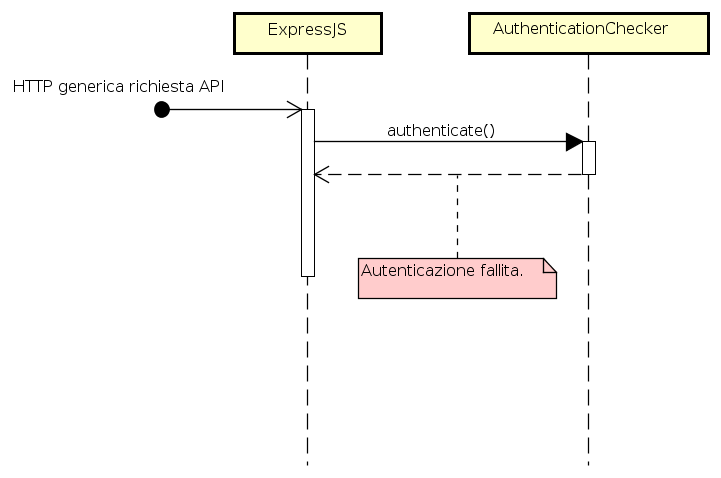
\includegraphics[width=0.8\textwidth]{res/sections/backend/sequence/autenticazioneFallita.png}
\caption{Autenticazione fallita}
\end{figure}
\paragraph{Livello minimo: MEMBER} \mbox{} \\
\textbf{Descrizione:} Tentativo di accesso ad una risorsa visibile solo a utenti con ruolo almeno MEMBER da parte di un utente GUEST.
\begin{figure}[H]
\centering
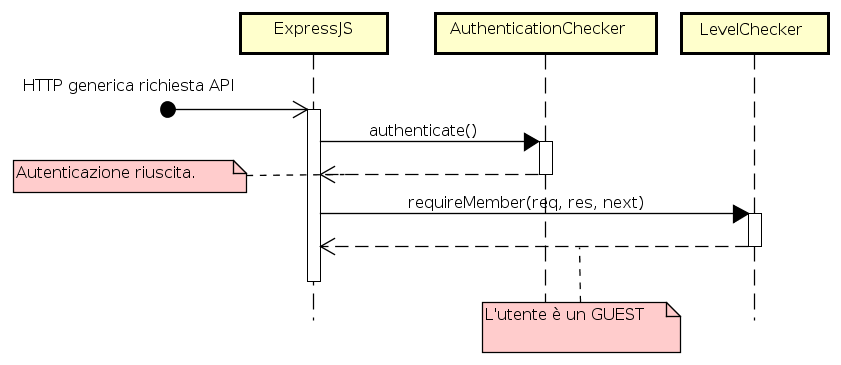
\includegraphics[width=0.8\textwidth]{res/sections/backend/sequence/requireMemberFallita.png}
\caption{Livello minimo MEMBER}
\end{figure}
\paragraph{Livello minimo: ADMIN} \mbox{} \\
\textbf{Descrizione:} Tentativo di accesso ad una risorsa visibile solo a utenti con ruolo almeno ADMIN da parte di un utente GUEST o MEMBER.
\begin{figure}[H]
\centering
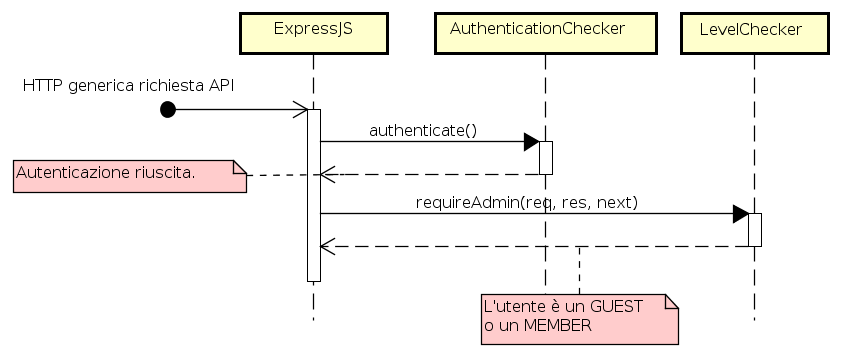
\includegraphics[width=0.8\textwidth]{res/sections/backend/sequence/requireAdminFallita.png}
\caption{Livello minimo ADMIN}
\end{figure}
\paragraph{Livello minimo: OWNER}  \mbox{} \\
\textbf{Descrizione:} Tentativo di accesso ad una risorsa visibile solo a utenti con ruolo almeno OWNER da parte di un utente GUEST, MEMBER o ADMIN.
\begin{figure}[H]
\centering
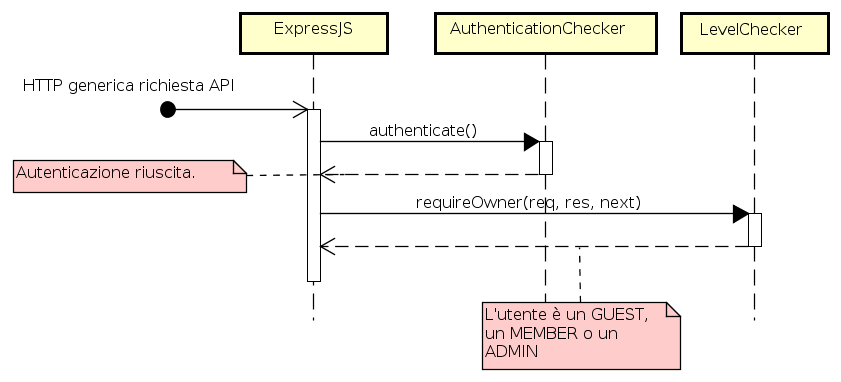
\includegraphics[width=0.8\textwidth]{res/sections/backend/sequence/requireOwnerFallita.png}
\caption{Livello minimo OWNER}
\end{figure}
\paragraph{Livello minimo: SUPERADMIN}  \mbox{} \\
\textbf{Descrizione:} Tentativo di accesso ad una risorsa accedibile solo da un SUPERADMIN da parte di un generico utente di MaaS.
\begin{figure}[H]
\centering
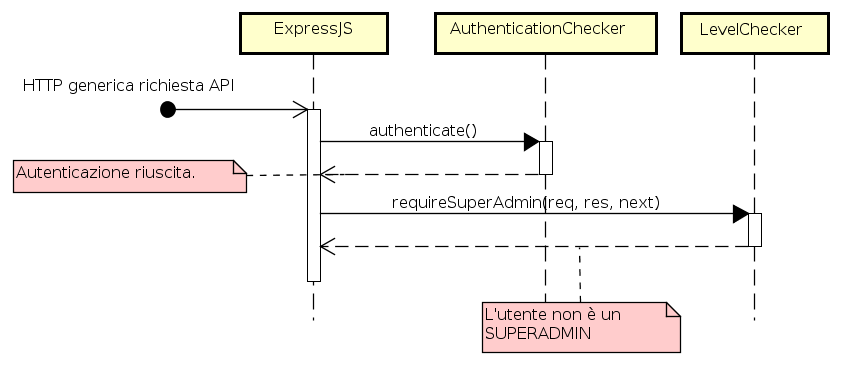
\includegraphics[width=0.8\textwidth]{res/sections/backend/sequence/requireSuperAdminFallita.png}
\caption{Livello minimo SUPERADMIN}
\end{figure}
\newpage
\subsection{API REST}
Di seguito sono descritte le API REST esposte dal server di MaaS. Si suppone che l'utente che richiede l'accesso alla risorsa descritta abbia i permessi necessari (ovvero che sia autenticato e che il suo ruolo sia conforme a quanto indicato). Qualora questo non fosse vero si ricadrebbe in uno degli scenari esposti precedentemente.
\subsubsection{Senza autenticazione}
\paragraph{Login}\mbox{}\\
\textbf{Tipologia:} POST \\
\textbf{API:} /api/login \\
\textbf{Descrizione:} Necessita di una richiesta con body contenente email e password dell'utente. \\
\textbf{Scenario:} 
\begin{figure}[H]
\centering
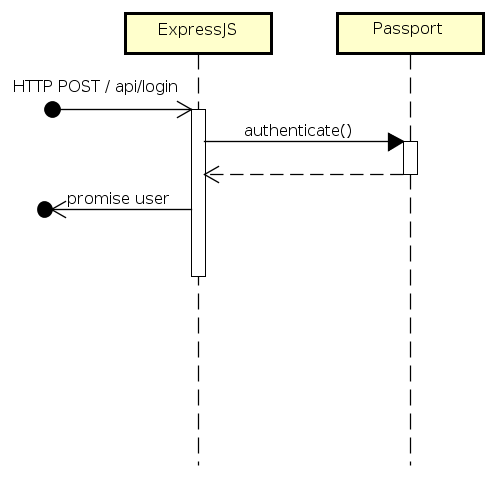
\includegraphics[width=0.8\textwidth]{res/sections/backend/sequence/(POST)login.png}
\caption{Scenario del login}
\end{figure}

\newpage
\paragraph{Registrazione}\mbox{}\\
\textbf{Tipologia:} POST \\
\textbf{API:} /api/register/:unique\_code \\
\textbf{Descrizione:} Metodo per la creazione di un utente invitato da una company. Necessita di una richiesta con body contenete le informazioni per la creazione completa di un utente \\
\textbf{Scenario:} 
\begin{figure}[H]
\centering
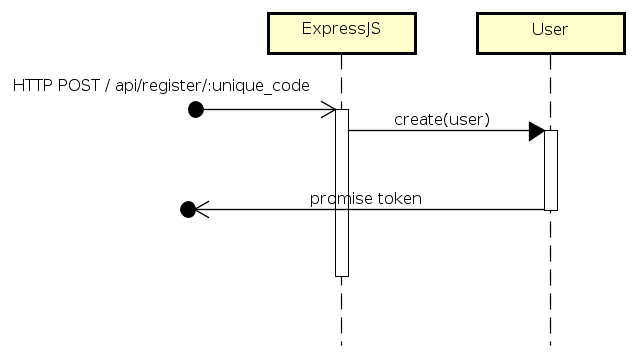
\includegraphics[width=0.8\textwidth]{res/sections/backend/sequence/(POST)register.png}
\caption{Scenario della registrazione}
\end{figure}

\newpage
\paragraph{Creazione Company}\mbox{}\\
\textbf{Tipologia:} POST \\
\textbf{API:} /api/companies \\
\textbf{Descrizione:} Necessita di una richiesta con body contenente le informazioni relative alla company e alla creazione del profilo del suo Owner. \\
\textbf{Scenario:} 
\begin{figure}[H]
\centering
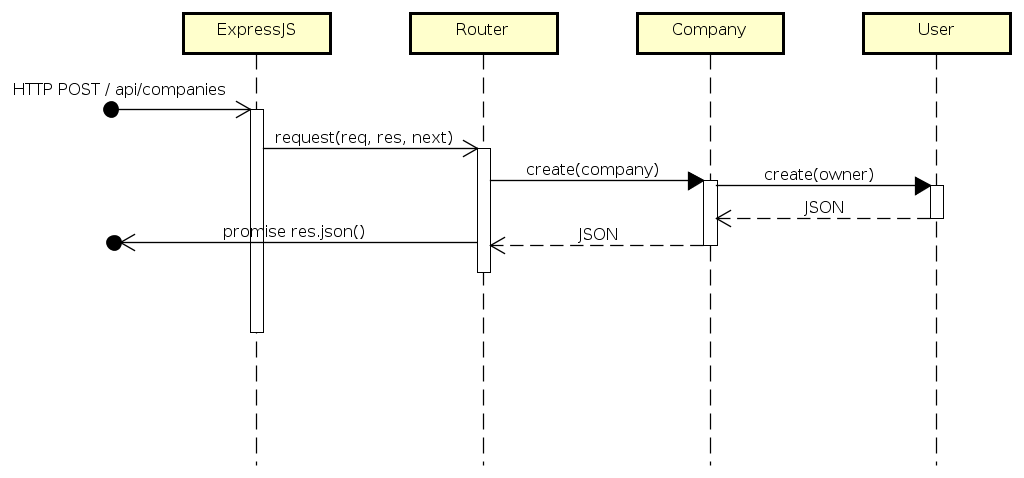
\includegraphics[width=0.8\textwidth]{res/sections/backend/sequence/(POST)company.png}
\caption{Scenario della creazione company}
\end{figure}

\newpage
\subsubsection{User}
\paragraph{Utenti di una company}\mbox{}\\
\textbf{Tipologia:} GET \\
\textbf{API:} /api/companies/:company\_id/users \\
\textbf{Livello di accesso minimo:} MEMBER \\
\textbf{Descrizione:} Ritorna un array di JSON contenenti i profili degli utenti della company. \\
\textbf{Scenario:} 
\begin{figure}[H]
\centering
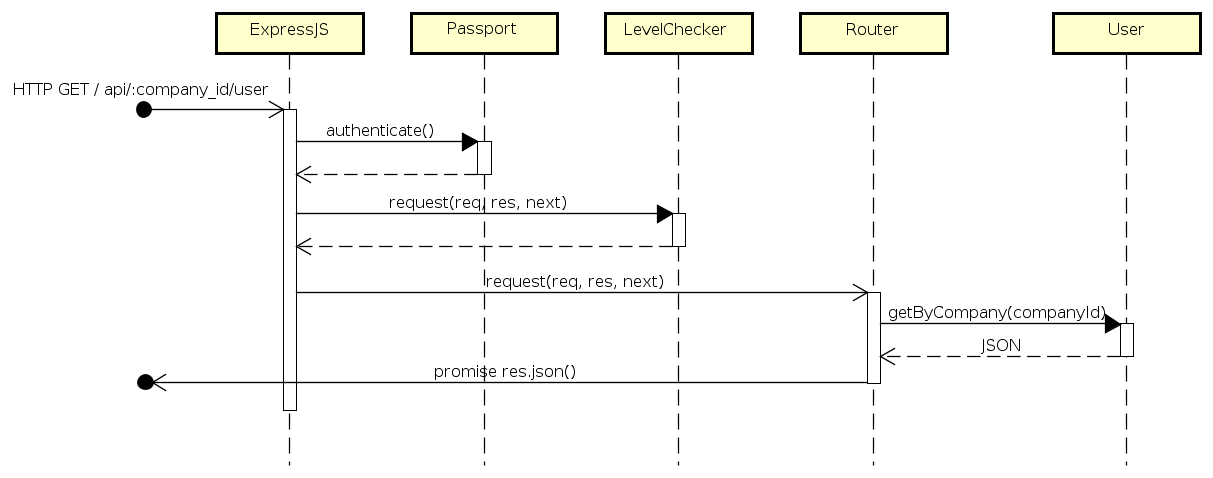
\includegraphics[width=0.8\textwidth]{res/sections/backend/sequence/(GET)user.png}
\caption{Scenario della ricerca utenti di una company specifica}
\end{figure}

\newpage
\paragraph{Inserimento utente}\mbox{}\\
\textbf{Tipologia:} POST \\
\textbf{API:} /api/companies/:company\_id/users \\
\textbf{Livello di accesso minimo:} OWNER \\
\textbf{Descrizione:} Necessita di una richiesta con body contenente l'email e il livello di accesso dell'utente.\\
\textbf{Scenario:} 
\begin{figure}[H]
\centering
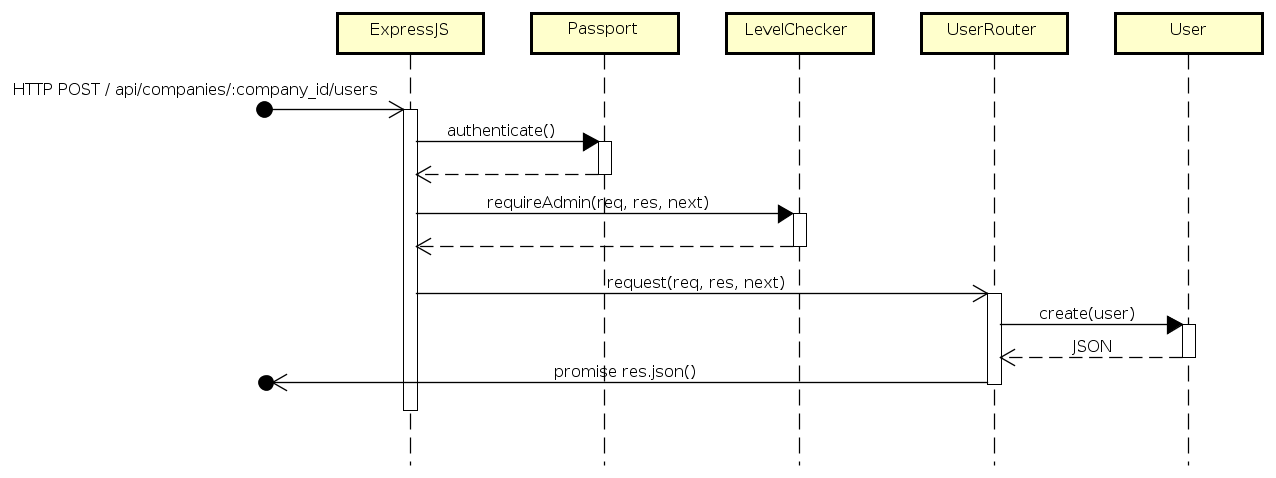
\includegraphics[width=0.8\textwidth]{res/sections/backend/sequence/(POST)user.png}
\caption{Scenario dell'inserimento utente in una company}
\end{figure}

\newpage
\paragraph{Aggiornamento delle credenziali utente}\mbox{}\\
\textbf{Tipologia:} PUT \\
\textbf{API:} /api/companies/:company\_id/users/:user\_id/credentials \\
\textbf{Livello di accesso minimo:} GUEST \\
\textbf{Descrizione:} Metodo per la modifica delle credenziali di accesso di un utente. Un utente ha il permesso di cambiare solo le proprie credenziali. \\
\textbf{Scenario:} 
\begin{figure}[H]
\centering
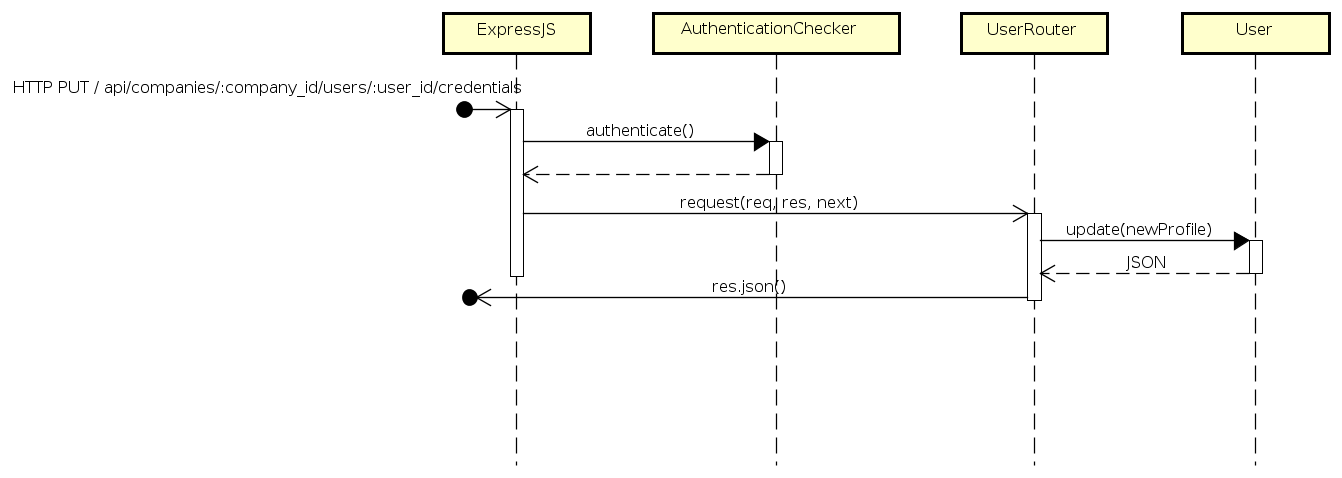
\includegraphics[width=0.8\textwidth]{res/sections/backend/sequence/(PUT)credenzialiUtente.png}
\caption{Scenario dell'aggiornamento delle credenziali di un utente}
\end{figure}

\newpage
\paragraph{Cancellazione utente}\mbox{}\\
\textbf{Tipologia:} DELETE \\
\textbf{API:} /api/companies/:company\_id/users/:user\_id \\
\textbf{Livello di accesso minimo:} OWNER \\
\textbf{Descrizione:} Ritorna un messaggio di conferma dell'avvenuta cancellazione. \\
\textbf{Scenario:} 
\begin{figure}[H]
\centering
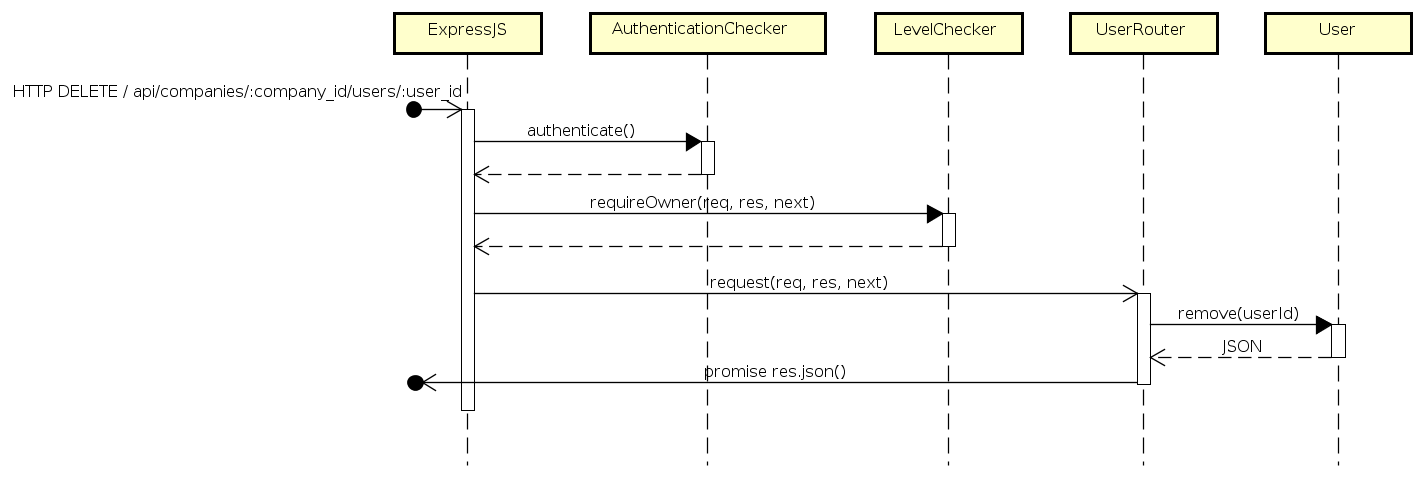
\includegraphics[width=0.8\textwidth]{res/sections/backend/sequence/(DELETE)user.png}
\caption{Scenario della cancellazione utente da una company}
\end{figure}

\newpage
\subsubsection{Company}
\paragraph{Dati di una company}\mbox{}\\
\textbf{Tipologia:} GET \\
\textbf{API:} /api/companies/:company\_id/ \\
\textbf{Livello di accesso minimo:} GUEST \\
\textbf{Descrizione:} Ritorna le informazioni generali di una company \\
\textbf{Scenario:} 
\begin{figure}[H]
\centering
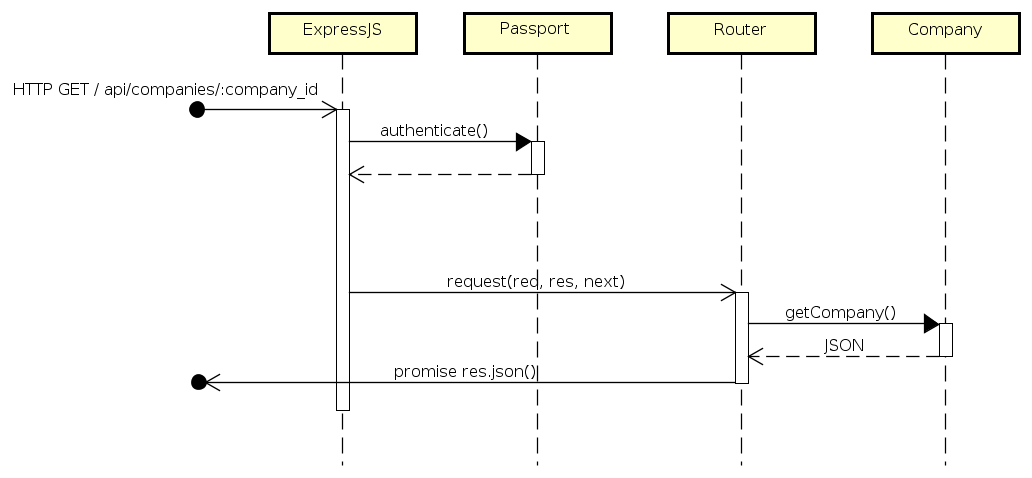
\includegraphics[width=0.8\textwidth]{res/sections/backend/sequence/(GET)company.png}
\caption{Scenario di ottenimento dei dati di una company}
\end{figure}

\newpage
\paragraph{Aggiornamento dei dati di una company}\mbox{}\\
\textbf{Tipologia:} PUT \\
\textbf{API:} /api/companies/:company\_id/ \\
\textbf{Livello di accesso minimo:} ADMIN \\
\textbf{Descrizione:} Necessita di una richiesta con body contenente le modifiche da apportare ai dati della company. \\
\textbf{Scenario:} 
\begin{figure}[H]
\centering
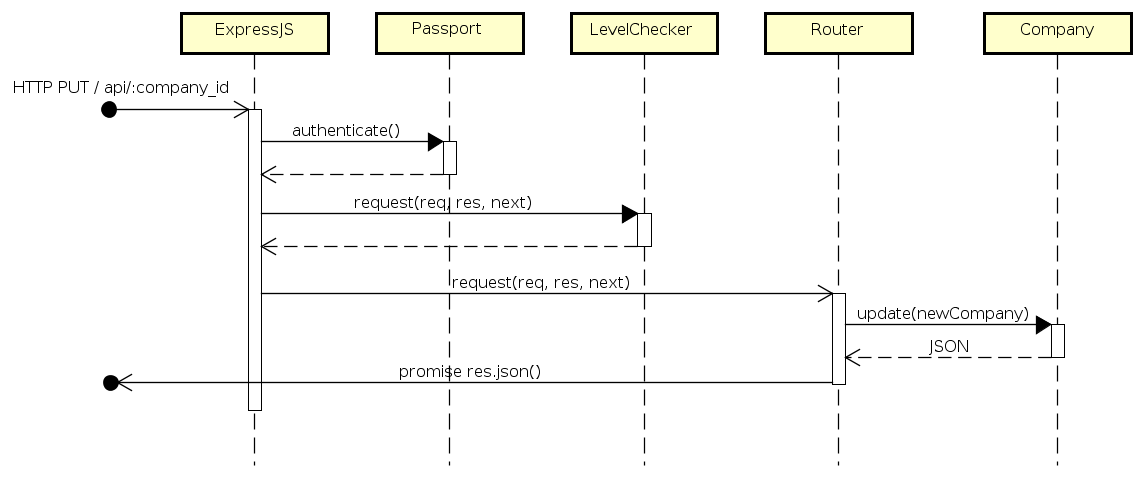
\includegraphics[width=0.8\textwidth]{res/sections/backend/sequence/(PUT)company.png}
\caption{Scenario dell'aggiornamento dei dati di una company}
\end{figure}

\newpage
\paragraph{Cancellazione di una company}\mbox{}\\
\textbf{Tipologia:} DELETE \\
\textbf{API:} /api/companies/:company\_id/ \\
\textbf{Livello di accesso minimo:} OWNER \\
\textbf{Descrizione:} Ritorna un messaggio di avvenuta cancellazione. \\
\textbf{Scenario:} 
\begin{figure}[H]
\centering
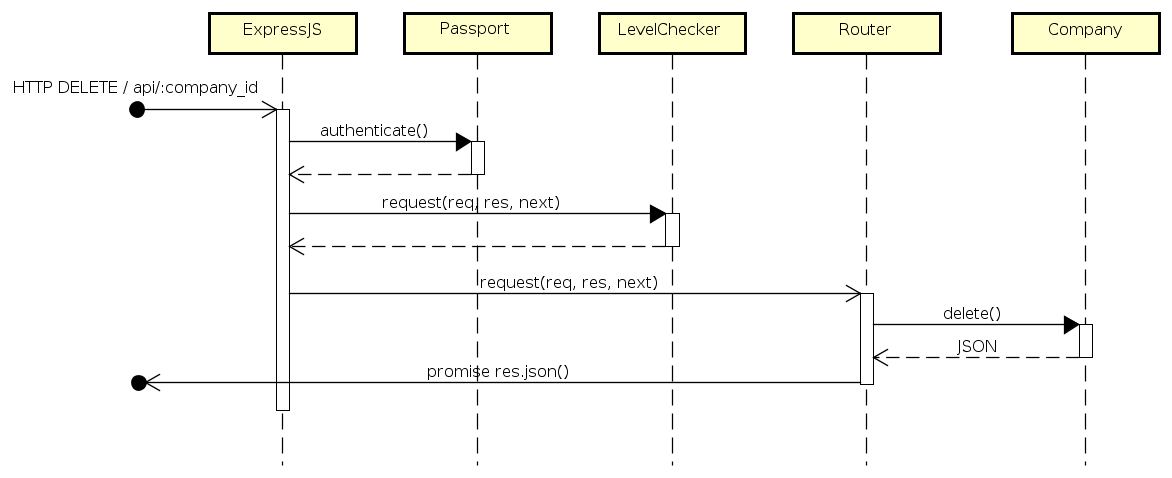
\includegraphics[width=0.8\textwidth]{res/sections/backend/sequence/(DELETE)company.png}
\caption{Scenario della cancellazione di una company}
\end{figure}

\newpage
\subsubsection{DSL}
\paragraph{Elenco delle specifiche DSL}\mbox{}\\
\textbf{Tipologia:} GET \\
\textbf{API:} /api/companies/:company\_id/DSLs \\
\textbf{Livello di accesso minimo:} GUEST \\
\textbf{Descrizione:} Ritorna un array contenente le specifiche DSL alle quali l'utente ha accesso in formato JSON. \\
\textbf{Scenario:} 
\begin{figure}[H]
\centering
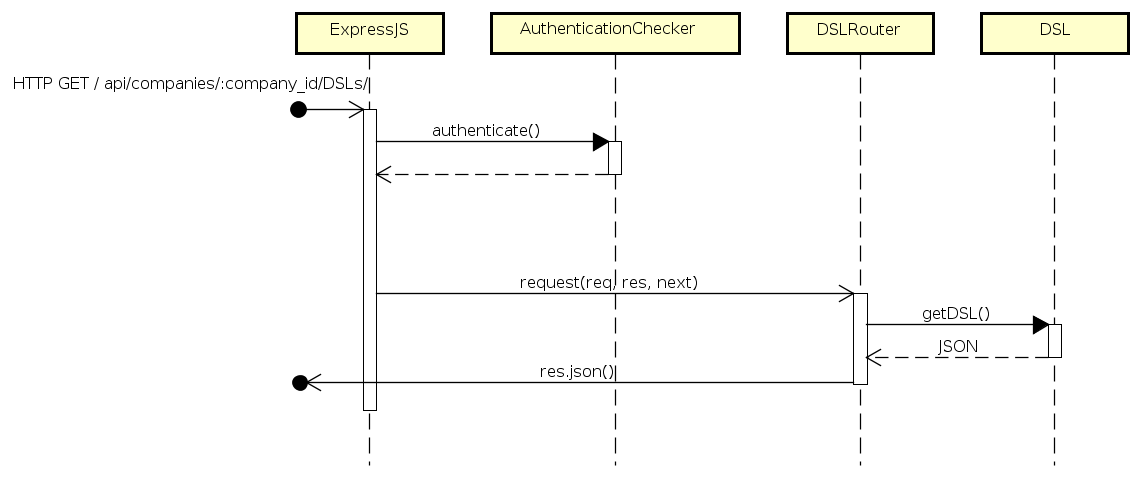
\includegraphics[width=0.8\textwidth]{res/sections/backend/sequence/(GET)dsl.png}
\caption{Scenario dell'elenco delle specifiche DSL}
\end{figure}

\newpage
\paragraph{Lettura del codice di una specifica DSL}\mbox{}\\
\textbf{Tipologia:} GET \\
\textbf{API:} /api/companies/:company\_id/DSLs/:dsl\_id \\
\textbf{Livello di accesso minimo:} MEMBER \\
\textbf{Descrizione:} Ritorna il codice della specifica DSL richiesta in formato JSON. \\
\textbf{Scenario:} 
\begin{figure}[H]
\centering
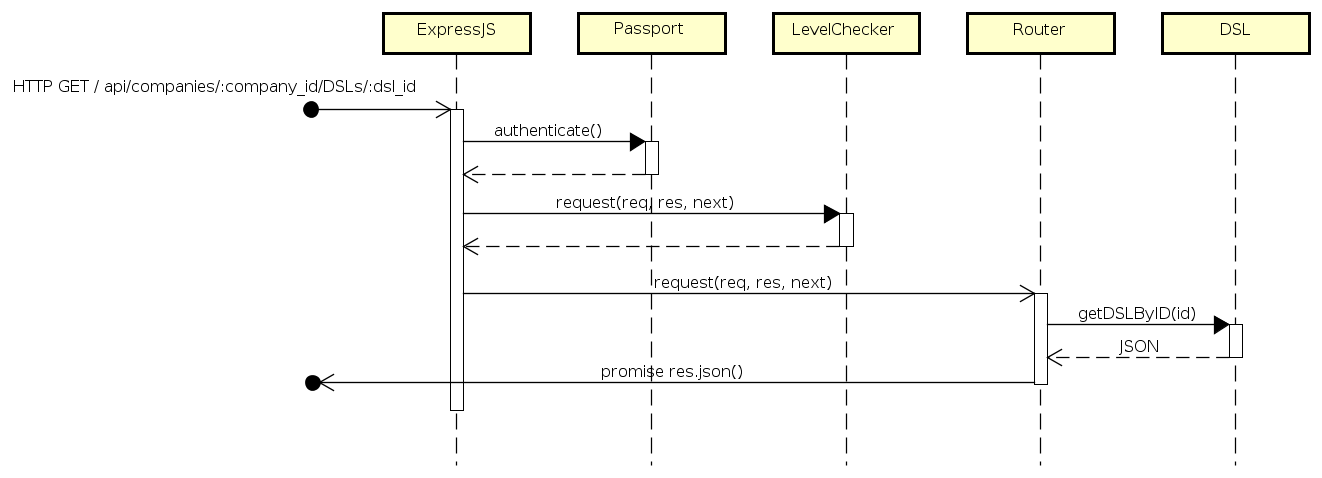
\includegraphics[width=0.8\textwidth]{res/sections/backend/sequence/(GET)dslByID.png}
\caption{Scenario della lettura del codice di una specifica DSL}
\end{figure}

\newpage
\paragraph{Aggiunta di una specifica DSL}\mbox{}\\
\textbf{Tipologia:} POST \\
\textbf{API:} /api/companies/:company\_id/DSLs \\
\textbf{Livello di accesso minimo:} MEMBER \\
\textbf{Descrizione:} Necessita di una richiesta con body contenente i dati necessari alla creazione della DSL. \\
\textbf{Scenario:} 
\begin{figure}[H]
\centering
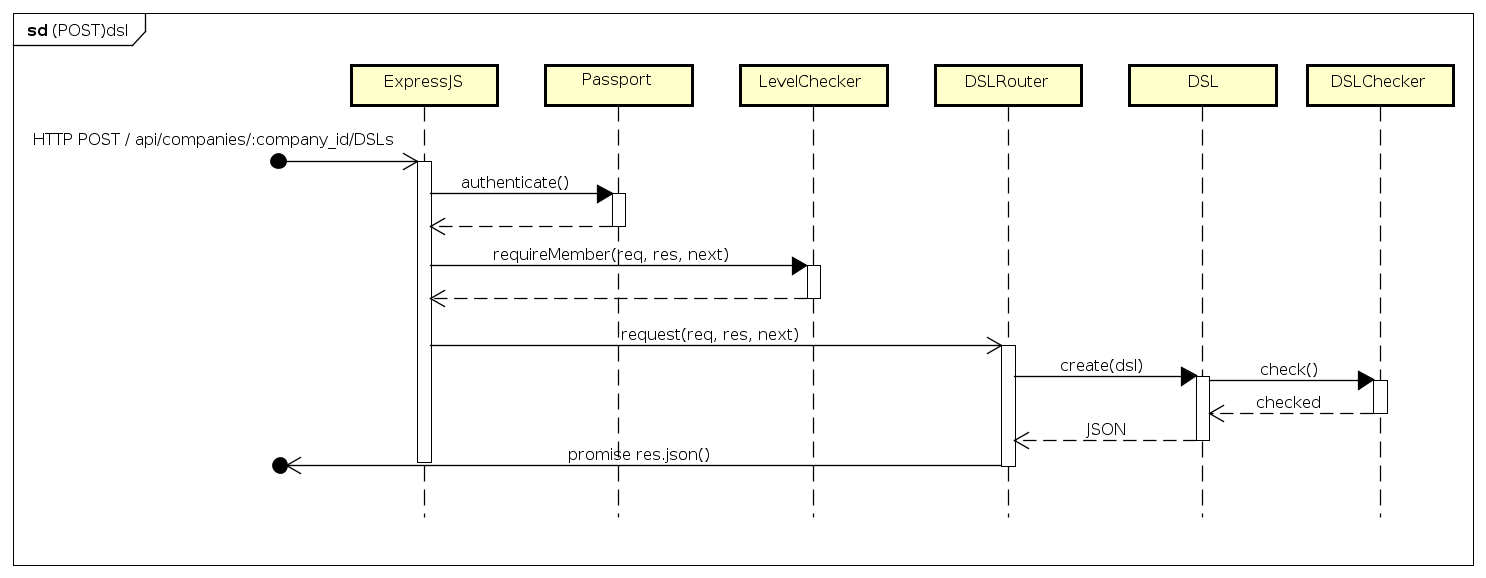
\includegraphics[width=0.8\textwidth]{res/sections/backend/sequence/(POST)dsl.png}
\caption{Scenario della creazione di una specifica DSL}
\end{figure}

\newpage
\paragraph{Aggiornamento del codice di una specifica DSL}\mbox{}\\
\textbf{Tipologia:} PUT \\
\textbf{API:} /api/companies/:company\_id/DSLs/:dsl\_id \\
\textbf{Livello di accesso minimo:} MEMBER \\
\textbf{Descrizione:} Necessita di una richiesta con body contenente i dati necessari alla modifica della DSL specificata da dsl\_id. \\
\textbf{Scenario:}
\begin{figure}[H]
\centering
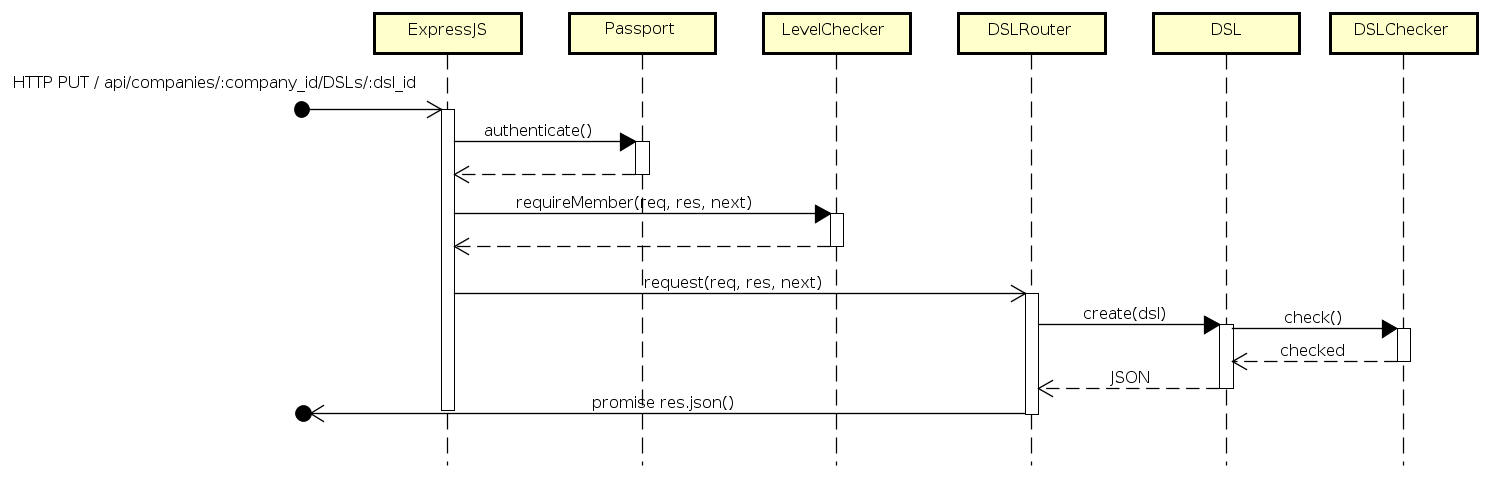
\includegraphics[width=0.8\textwidth]{res/sections/backend/sequence/(PUT)dsl.png}
\caption{Scenario dell'aggiornamento del codice di una specifica DSL}
\end{figure}

\newpage
\paragraph{Cancellazione di una specifica DSL}\mbox{}\\
\textbf{Tipologia:} DELETE \\
\textbf{API:} /api/companies/:company\_id/DSLs/:dsl\_id \\
\textbf{Livello di accesso minimo:} MEMBER \\
\textbf{Descrizione:} Ritorna un messaggio in formato JSON di avvenuta cancellazione. \\
\textbf{Scenario:} 
\begin{figure}[H]
\centering
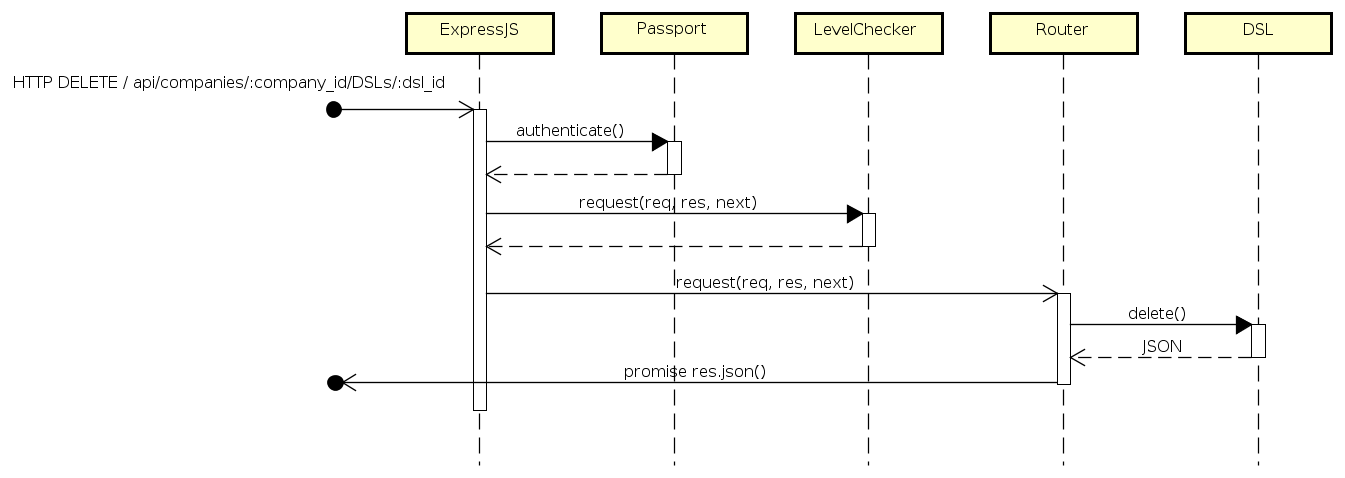
\includegraphics[width=0.8\textwidth]{res/sections/backend/sequence/(DELETE)dsl.png}
\caption{Scenario della cancellazione di una specifica DSL}
\end{figure}

\newpage
\paragraph{Ottenimento della dashboard di un utente}\mbox{}\\
\textbf{Tipologia:} GET \\
\textbf{API:} /api/companies/:company\_id/users/:user\_id/dashboard \\
\textbf{Livello di accesso minimo:} GUEST \\
\textbf{Descrizione:} Ritorna la dashboard di un utente definita da una DSL. \\
\textbf{Scenario:}  
\begin{figure}[H]
\centering
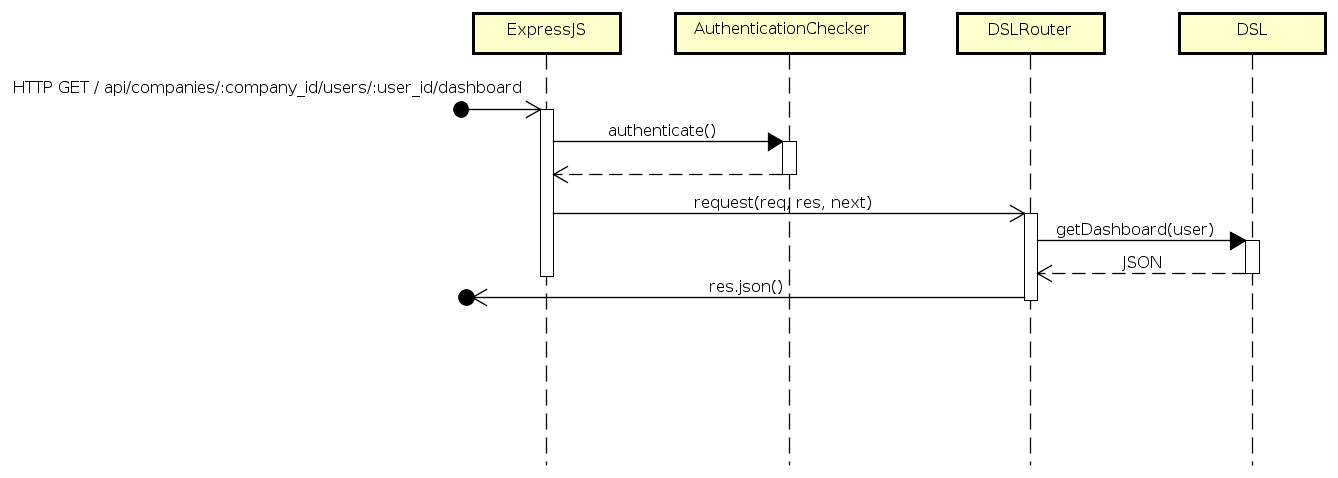
\includegraphics[width=0.8\textwidth]{res/sections/backend/sequence/(GET)dashboard.png}
\caption{Scenario dell'ottenimento della dashboard di un utente}
\end{figure}

\newpage
\paragraph{Esecuzione di una specifica DSL}\mbox{}\\
\textbf{Tipologia:} GET \\
\textbf{API:} /api/companies/:company\_id/DSLs/:dsl\_id/execute \\
\textbf{Livello di accesso minimo:} GUEST \\
\textbf{Descrizione:} Ritorna un JSON contenente i dati richiesti dalla specifica DSL e la struttura su cui inserire i dati. \\
\textbf{Scenario:} 
\begin{figure}[H]
\centering
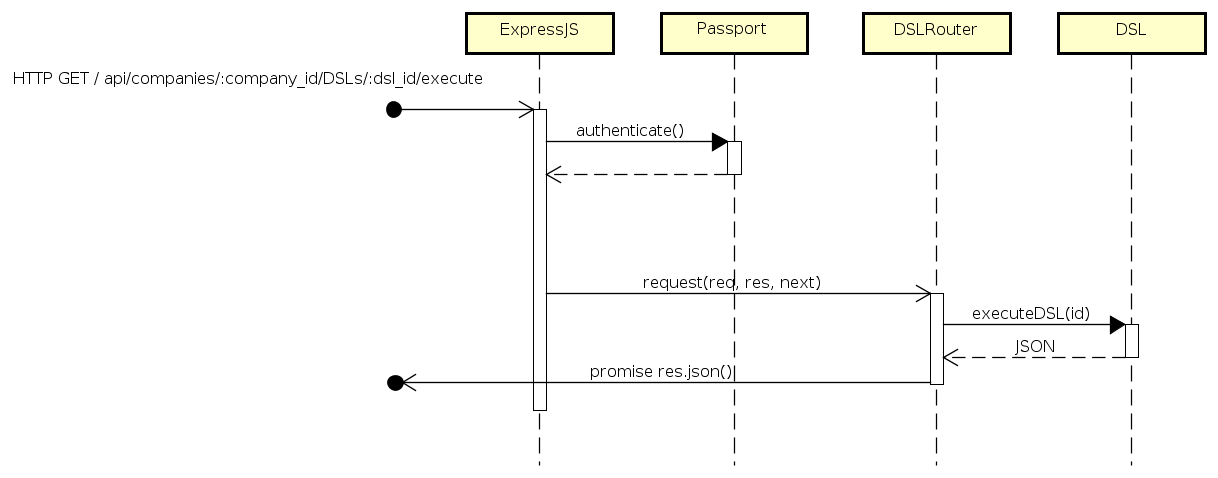
\includegraphics[width=0.8\textwidth]{res/sections/backend/sequence/(GET)dslByIDex.png}
\caption{Scenario dell'esecuzione di una specifica DSL}
\end{figure}

\newpage
\subsubsection{Database}
\paragraph{Elenco dei database della company}\mbox{}\\
\textbf{Tipologia:} GET \\
\textbf{API:} /api/companies/:company\_id/databases \\
\textbf{Livello di accesso minimo:} MEMBER \\
\textbf{Descrizione:} Ritorna un array contenente i nomi e gli id di ciascun database. \\
\textbf{Scenario:}
\begin{figure}[H]
\centering
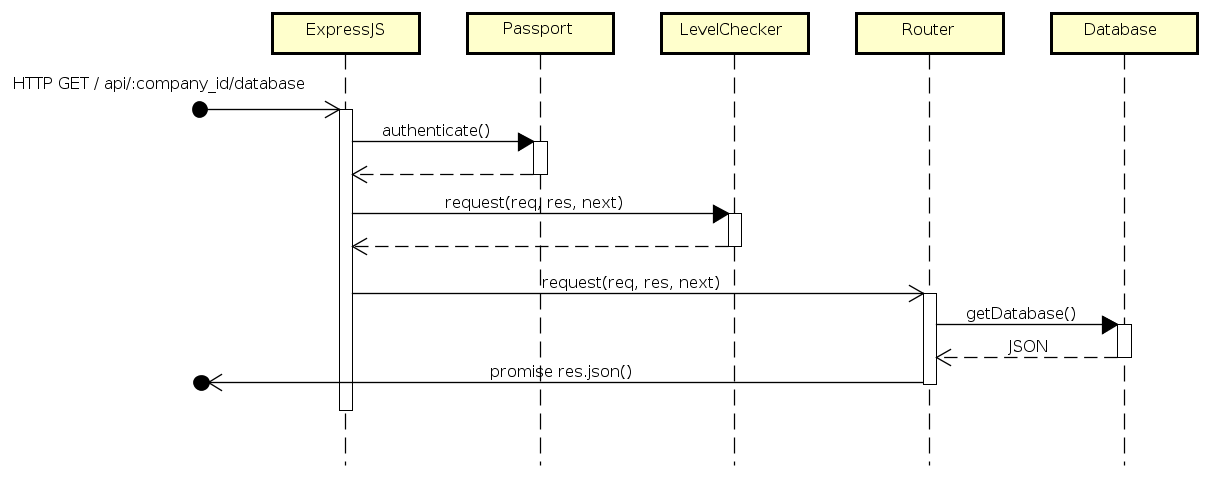
\includegraphics[width=0.8\textwidth]{res/sections/backend/sequence/(GET)database.png}
\caption{Scenario dell'elenco dei database propri della company}
\end{figure}

\newpage
\paragraph{Visualizzazione dati di un database}\mbox{}\\
\textbf{Tipologia:} GET \\
\textbf{API:} /api/companies/:company\_id/databases/:database\_id \\
\textbf{Livello di accesso minimo:} ADMIN \\
\textbf{Descrizione:} Ritorna tutte le informazioni relative al database richiesto. \\
\textbf{Scenario:} 
\begin{figure}[H]
\centering
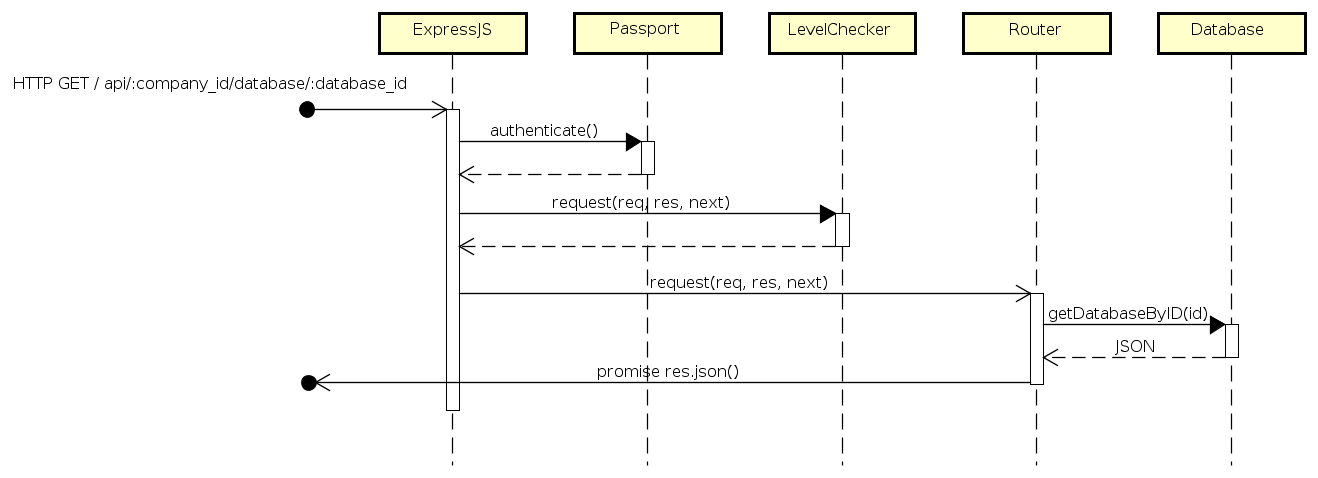
\includegraphics[width=0.8\textwidth]{res/sections/backend/sequence/(GET)databaseById.png}
\caption{Scenario della visualizzazione dei dati di un database}
\end{figure}

\newpage
\paragraph{Aggiunta di un database}\mbox{}\\
\textbf{Tipologia:} POST \\
\textbf{API:} /api/companies/:company\_id/databases \\
\textbf{Livello di accesso minimo:} ADMIN \\
\textbf{Descrizione:} Necessita di una richiesta con body contenete i dati relativi alla connessione del nuovo database. \\
\textbf{Scenario:}
\begin{figure}[H]
\centering
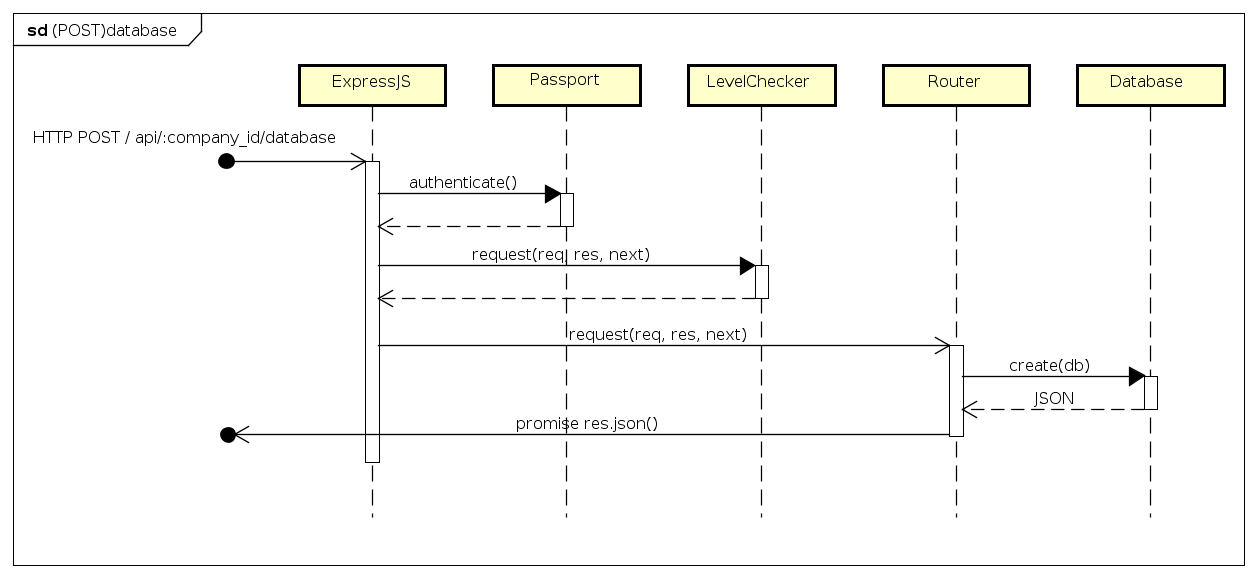
\includegraphics[width=0.8\textwidth]{res/sections/backend/sequence/(POST)database.png}
\caption{Scenario della creazione di una specifica DSL}
\end{figure}

\newpage
\paragraph{Aggiornamento di un database}\mbox{}\\
\textbf{Tipologia:} PUT \\
\textbf{API:} /api/companies/:company\_id/databases/:database\_id \\
\textbf{Livello di accesso minimo:} ADMIN \\
\textbf{Descrizione:} Metodo per aggiornare le informazioni relative alla connessione al database o per aggiornare l'elenco delle collezioni. \\
\textbf{Scenario:}
\begin{figure}[H]
\centering
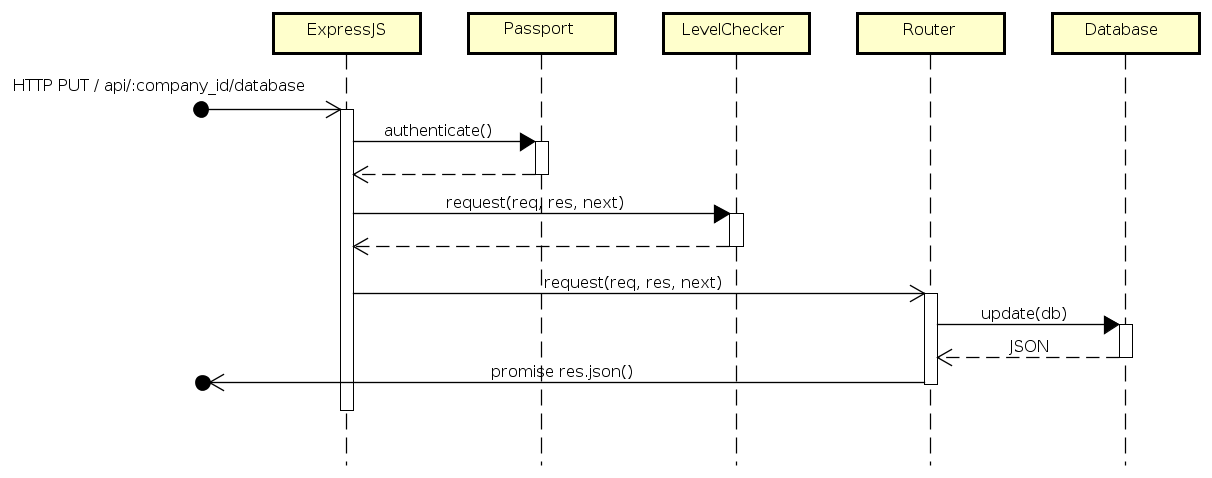
\includegraphics[width=0.8\textwidth]{res/sections/backend/sequence/(PUT)database.png}
\caption{Scenario dell'aggiornamento di un database}
\end{figure}

\newpage
\paragraph{Cancellazione di un database}\mbox{}\\
\textbf{Tipologia:} DELETE \\
\textbf{API:} /api/companies/:company\_id/databases/:database\_id \\
\textbf{Livello di accesso minimo:} ADMIN \\
\textbf{Descrizione:} Elimina il database selezionato e tutte le DSL che lo utilizzano. \\
\textbf{Scenario:} 
\begin{figure}[H]
\centering
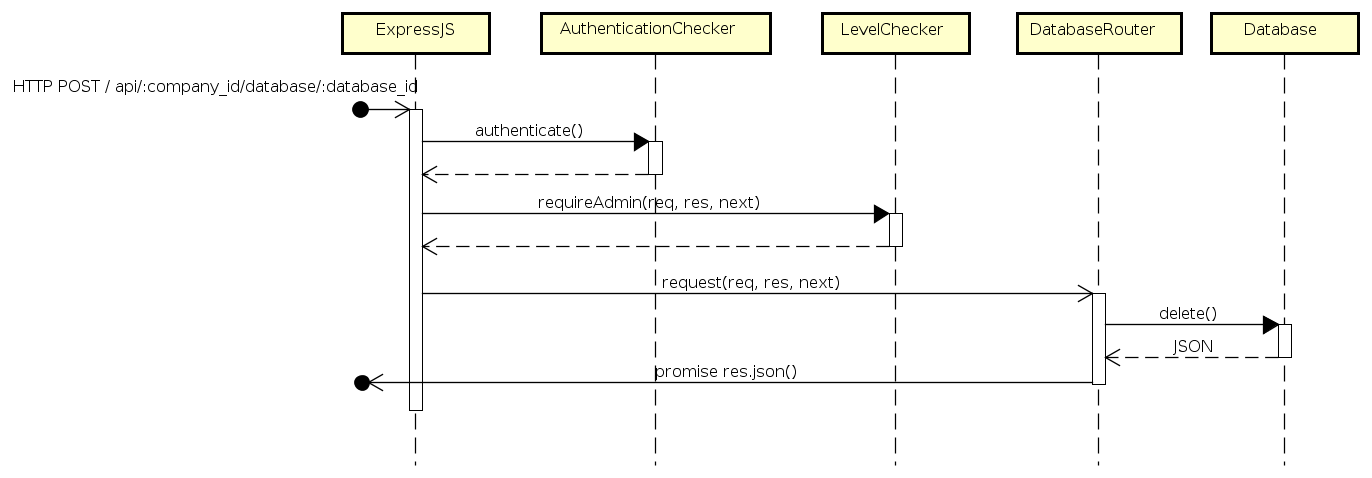
\includegraphics[width=0.8\textwidth]{res/sections/backend/sequence/(DELETE)database.png}
\caption{Scenario della cancellazione di un database}
\end{figure}

\newpage
\paragraph{Visualizzazione collections di un database} \mbox{}\\
\textbf{Tipologia:} GET \\
\textbf{API:} /api/companies/:company\_id/databases/:database\_id/collections \\
\textbf{Livello di accesso minimo:} MEMBER \\
\textbf{Descrizione:} Ritorna un array di collection relative ad un database a cui l'utente ha accesso. \\
\textbf{Scenario:} 
\begin{figure}[H]
\centering
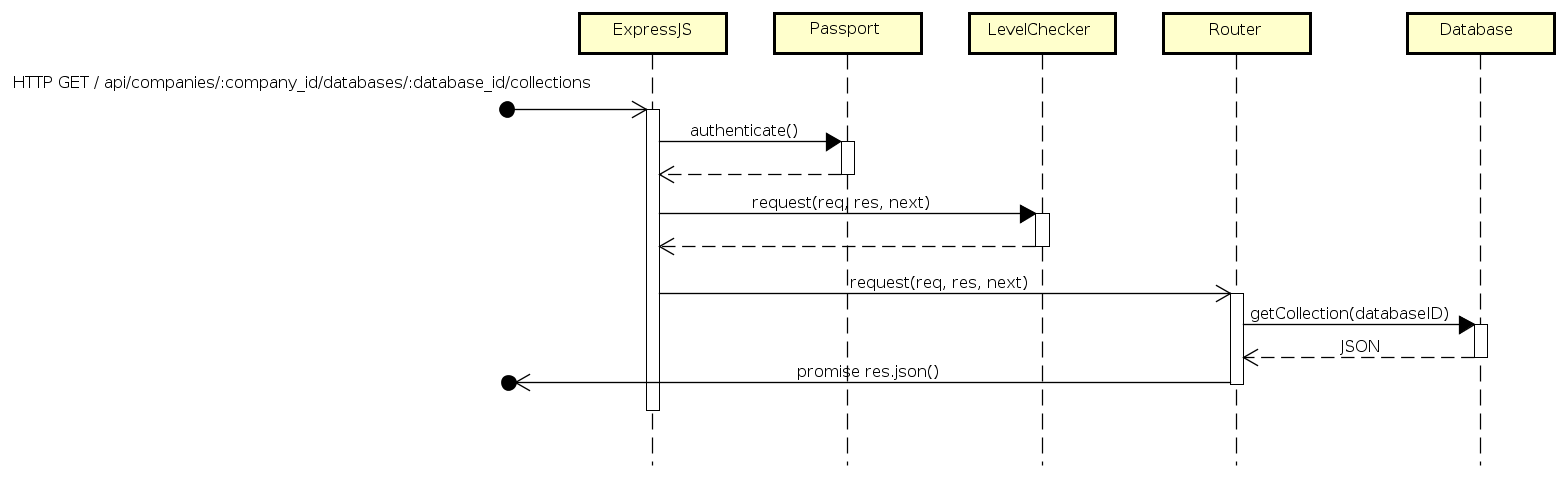
\includegraphics[width=0.8\textwidth]{res/sections/backend/sequence/(GET)collection.png}
\caption{Scenario della visualizzazione collections di un database}
\end{figure}

\newpage
\subsubsection{Super admin}
\paragraph{Ottenimento informazioni delle companies}\mbox{}\\
\textbf{Tipologia:} GET \\
\textbf{API:} /api/admin/companies \\
\textbf{Descrizione:} Restituisce un array di JSON contenenti le informazioni relative alle company presenti nell'applicazione. \\
\textbf{Scenario:} 
\begin{figure}[H]
\centering
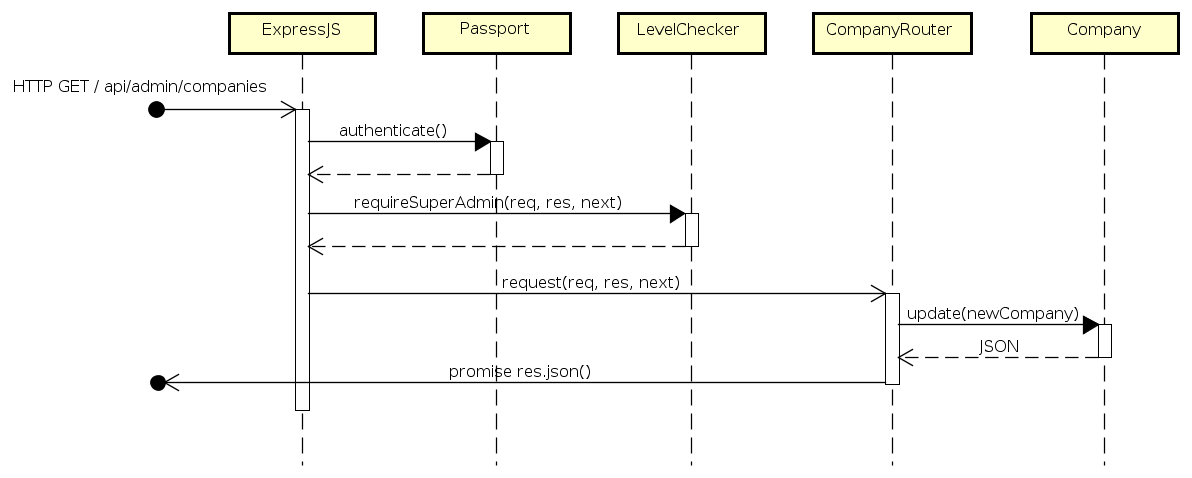
\includegraphics[width=0.8\textwidth]{res/sections/backend/sequence/(GET)companySA.png}
\caption{Scenario dell'ottenimento informazioni delle companies}
\end{figure}

\newpage
\paragraph{Aggiunta di un super admin}\mbox{}\\
\textbf{Tipologia:} POST \\
\textbf{API:} /api/admin/superadmins \\
\textbf{Descrizione:} Necessita di una richiesta con body contenente le informazioni relative al superadmin da creare. \\
\textbf{Scenario:} 
\begin{figure}[H]
\centering
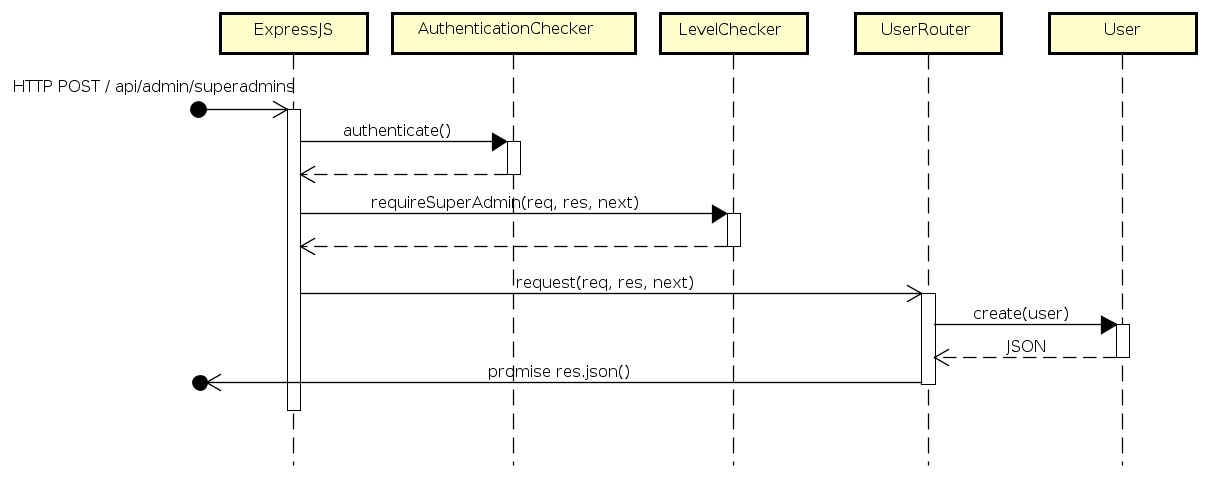
\includegraphics[width=0.8\textwidth]{res/sections/backend/sequence/(POST)superadmin.png}
\caption{Scenario dell'aggiunta di un super admin}
\end{figure}

\newpage
\paragraph{Aggiunta di un utente}\mbox{}\\
\textbf{Tipologia:} POST \\
\textbf{API:} /api/admin/companies/:company\_id/users \\
\textbf{Descrizione:} Necessita di una richiesta con body contenente le informazioni relative all'utente da creare per la company individuata da company\_id. \\
\textbf{Scenario:} 
\begin{figure}[H]
\centering
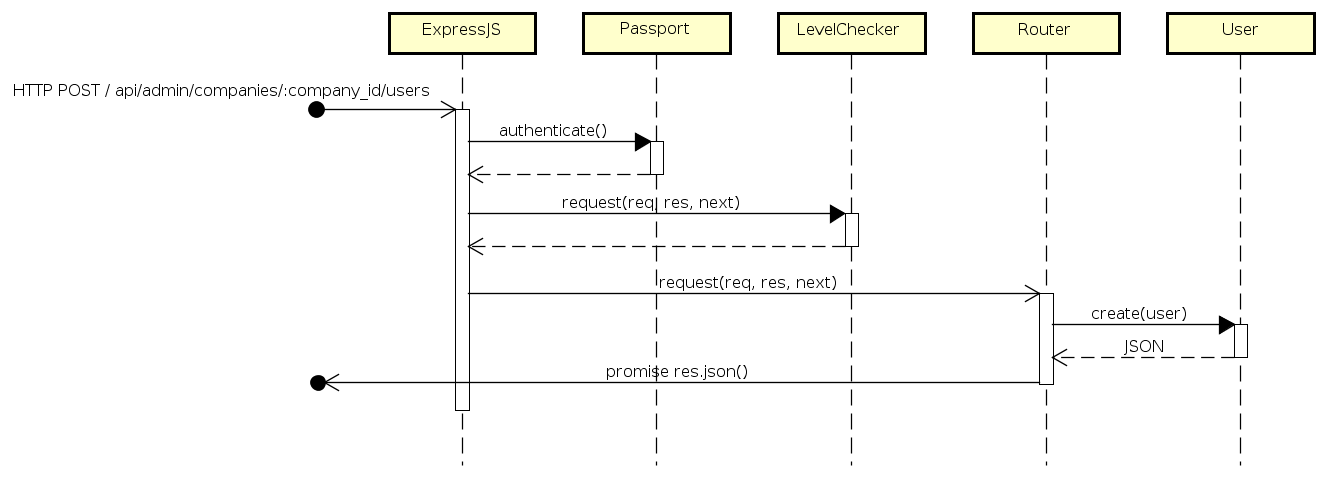
\includegraphics[width=0.8\textwidth]{res/sections/backend/sequence/(POST)userSA.png}
\caption{Scenario dell'aggiunta di un utente}
\end{figure}

\section{Editor}

Di seguito viengono elencati i casi d'uso per l'editor.

%\newpage da rimuovere?

\subsection{Casi d'Uso}


\subsubsection{UC-E}

    \begin{figure}[H]
      \begin{center}
        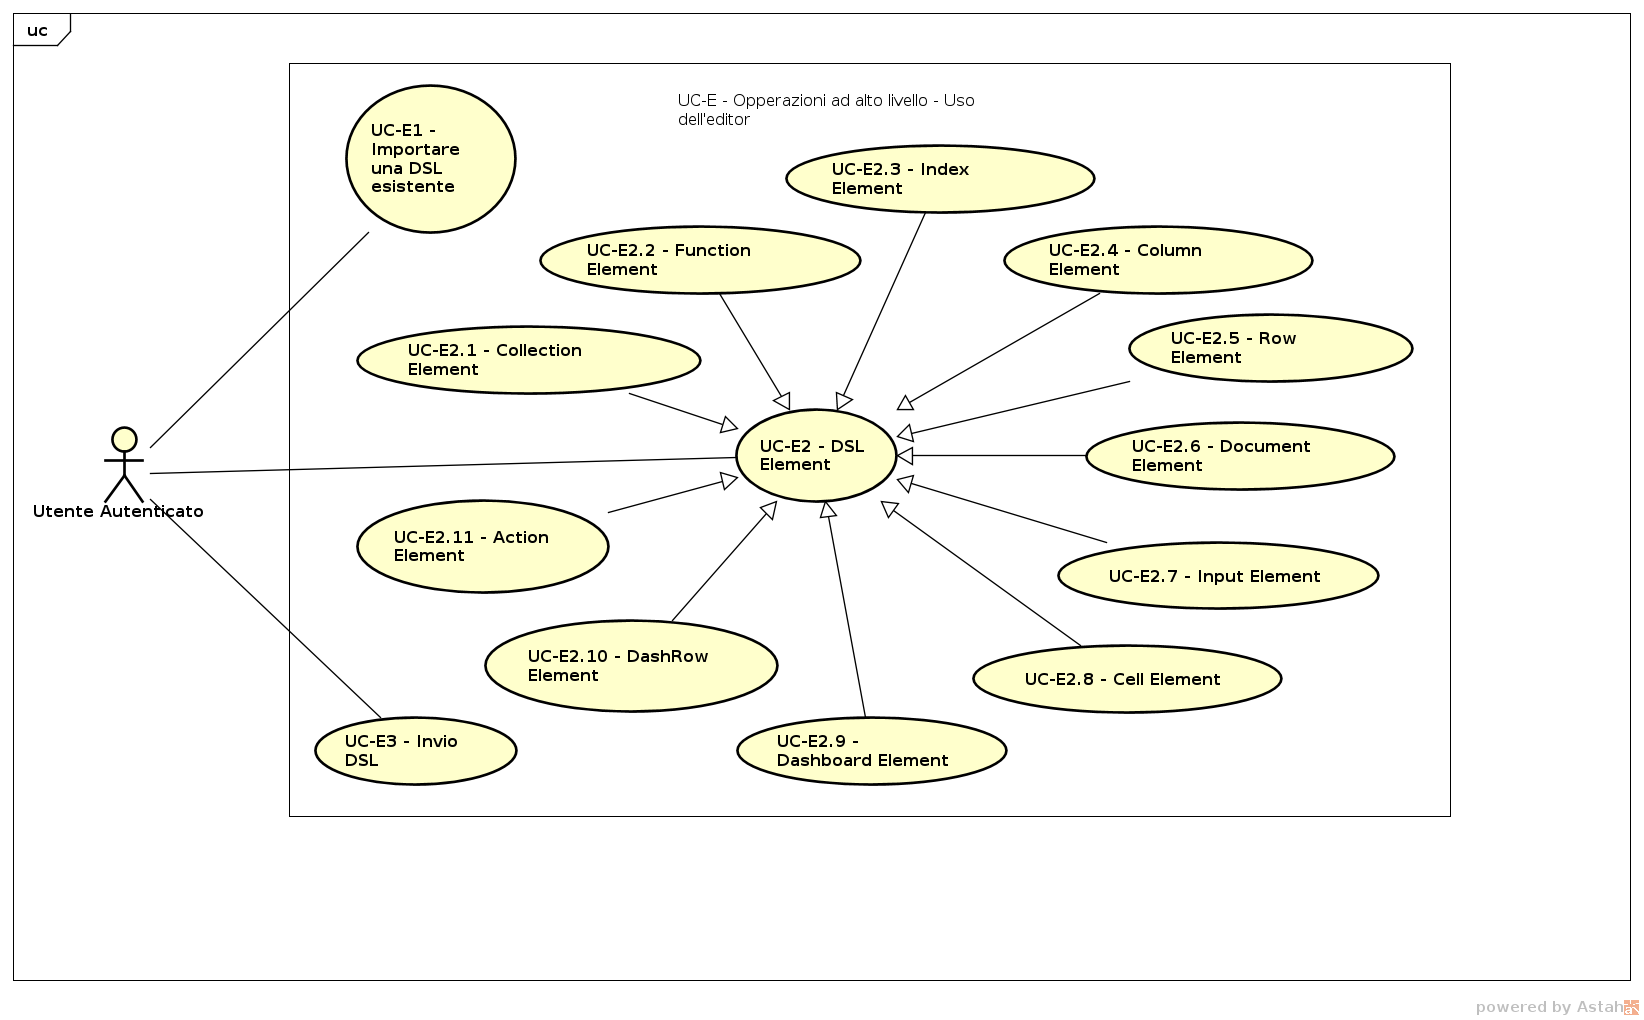
\includegraphics[width=12cm]{res/img/UCEditor/UC-E}
      \caption{UC-E - Operazioni ad alto livello - Uso dell'editor}
      \end{center} 
    \end{figure}    
    
    %Tabella 
    \begin{center}
      \bgroup
      \def\arraystretch{1.8}     
      \begin{longtable}{  p{3.5cm} | p{8cm} } 
        
        \hline
        \multicolumn{2}{ | c | }{ \cellcolor[gray]{0.9} \textbf{UC-E - Operazioni ad alto livello - Uso dell'editor}} \\ 
        \hline
        
        \textbf{Attori Primari} & Utente Autenticato, Ospite, Membro, Admin, Proprietario \\ 
        \textbf{Scopo e Descrizione} & 1. Importare un DSL esitente (UC-E1)
2. Manipolazione del DSL Element tramite l'interfaccia grafica dell'editor
3. Invio del DSL \\ 
        
        \textbf{Precondizioni}  & 1. Importare un DSL esitente (UC-E1)
2. Manipolazione del DSL Element tramite l'interfaccia grafica dell'editor
3. Invio del DSL \\ 
        
        \textbf{Postcondizioni} & L'utente ha utilizzato l'editor ed ha eseguito le azioni volute \\ 
        \textbf{Flusso Principale} & 1. Importare un DSL esistente
2. DSL element
3. Invio di un DSL \\
        \textbf{Estensioni} &  \\
        \textbf{Inclusioni} & 
      \end{longtable}
      \egroup
    \end{center} 


\subsubsection{UC-E2}

    \begin{figure}[H]
      \begin{center}
        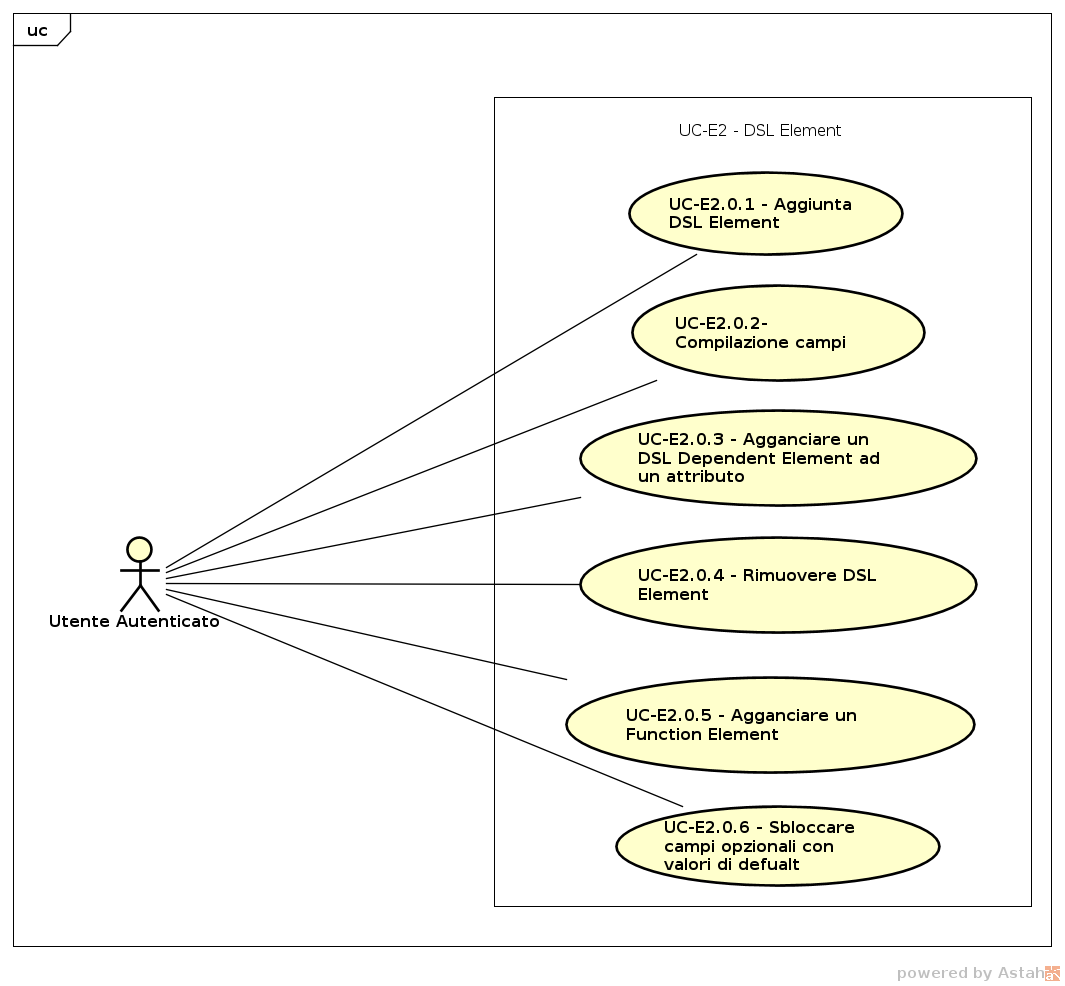
\includegraphics[width=12cm]{res/img/UCEditor/UC-E2-DSLElement}
      \caption{UC-E2 - DSL Element}
      \end{center} 
    \end{figure}    
    
    %Tabella 
    \begin{center}
      \bgroup
      \def\arraystretch{1.8}     
      \begin{longtable}{  p{3.5cm} | p{8cm} } 
        
        \hline
        \multicolumn{2}{ | c | }{ \cellcolor[gray]{0.9} \textbf{UC-E2 - DSL Element}} \\ 
        \hline
        
        \textbf{Attori Primari} & Utente Autenticato, Ospite, Membro, Admin, Proprietario \\ 
        \textbf{Scopo e Descrizione} & Il DSL element è la zona dove è possibile aggiungere, agganciare, sbloccare o rimuovere altri elementi del DSL. È possibile anche la compilazione dei campi. \\ 
        
        \textbf{Precondizioni}  & Il DSL element è la zona dove è possibile aggiungere, agganciare, sbloccare o rimuovere altri elementi del DSL. È possibile anche la compilazione dei campi. \\ 
        
        \textbf{Postcondizioni} & L'utente ha eseguito le sue operazioni sul DSL Element \\ 
        \textbf{Flusso Principale} & 1. Aggiunta DSL Element (UC-E2.0.1)
2. Compilazione campi (UC-E2.0.2)
3. Agganciare un DSL Dependent Element ad un attributo (UC-E2.0.3)
4. Rimuovere DSL Element (UC-E2.0.4)
5. Agganciare un Function Element (UC-E2.0.5)
6. Sbloccare campi opzionali con valori di default (UC-E2.0.6) \\
        \textbf{Estensioni} &  \\
        \textbf{Inclusioni} & 
      \end{longtable}
      \egroup
    \end{center} 


\subsubsection{UC-E2.0.1}

    %\begin{figure}[H]
    %  \begin{center}
    %    \includegraphics[width=12cm]{res/img/}
    %  \caption{UC-E2.0.1 - Aggiunta DSL Element}
    %  \end{center} 
    %\end{figure}    
    
    %Tabella 
    \begin{center}
      \bgroup
      \def\arraystretch{1.8}     
      \begin{longtable}{  p{3.5cm} | p{8cm} } 
        
        \hline
        \multicolumn{2}{ | c | }{ \cellcolor[gray]{0.9} \textbf{UC-E2.0.1 - Aggiunta DSL Element}} \\ 
        \hline
        
        \textbf{Attori Primari} & Utente Autenticato, Ospiete, Membro, Admin, Proprietario \\ 
        \textbf{Scopo e Descrizione} & L'utente ha la possibiltà di aggiungere un elemento DSL \\ 
        
        \textbf{Precondizioni}  & L'utente ha la possibiltà di aggiungere un elemento DSL \\ 
        
        \textbf{Postcondizioni} & L'utente ha aggiunto con successo un elemento DSL \\ 
        \textbf{Flusso Principale} &  \\
        \textbf{Estensioni} &  \\
        \textbf{Inclusioni} & 
      \end{longtable}
      \egroup
    \end{center} 
\subsubsection{UC-E2.0.2}

    %Tabella 
    \begin{center}
      \bgroup
      \def\arraystretch{1.8}     
      \begin{longtable}{  p{3.5cm} | p{8cm} } 
        
        \hline
        \multicolumn{2}{ | c | }{ \cellcolor[gray]{0.9} \textbf{UC-E2.0.2 - Compilazione campi}} \\ 
        \hline
        
        \textbf{Attori Primari} & Utente Autenticato, Ospite, Membro, Admin, Proprietario \\ 
        \textbf{Scopo e Descrizione} & L'utente ha la possibilit\`a di compilare i campi con del testo personalizzato \\ 
        
        \textbf{Precondizioni}  & L'utente ha la possibilit\`a di compilare i campi desiderati \\ 
        
        \textbf{Postcondizioni} & I campi desiderati dall'utente sono stati compilati con successo \\ 
        \textbf{Flusso Principale} &  \\
        \textbf{Estensioni} &  \\
        \textbf{Inclusioni} & 
      \end{longtable}
      \egroup
    \end{center}
\subsubsection{UC-E2.0.3}

    %Tabella 
    \begin{center}
      \bgroup
      \def\arraystretch{1.8}     
      \begin{longtable}{  p{3.5cm} | p{8cm} } 
        
        \hline
        \multicolumn{2}{ | c | }{ \cellcolor[gray]{0.9} \textbf{UC-E2.0.3 - Agganciare un DSL Dependent Element ad un attributo}} \\ 
        \hline
        
        \textbf{Attori Primari} & Utente Autenticato, Ospiete, Membro, Admin, Proprietario \\ 
        \textbf{Scopo e Descrizione} & Si da la possibilit\`a di agganciare un DSL Dependent Element ad un attributo. Questa azione \`e ripetibile diverse volte \\ 
        
        \textbf{Precondizioni}  & L'utente ha a disposizione un attributo e un DSL Dependent Element \\ 
        
        \textbf{Postcondizioni} & L'utente ha collegato con successo l'atributo e il DSL Dependent Element a disposizione \\ 
        \textbf{Flusso Principale} &  \\
        \textbf{Estensioni} &  \\
        \textbf{Inclusioni} & 
      \end{longtable}
      \egroup
    \end{center}
\subsubsection{UC-E2.0.4}

    %Tabella 
    \begin{center}
      \bgroup
      \def\arraystretch{1.8}     
      \begin{longtable}{  p{3.5cm} | p{8cm} } 
        
        \hline
        \multicolumn{2}{ | c | }{ \cellcolor[gray]{0.9} \textbf{UC-E2.0.4 - Rimuovere DSL Element}} \\ 
        \hline
        
        \textbf{Attori Primari} & Utente Autenticato, Ospite, Membro, Admin, Proprietario \\ 
        \textbf{Scopo e Descrizione} & \`E possibile rimuovere un DSL Element non pi\`u utilizzato o non pi\`u voluto \\ 
        
        \textbf{Precondizioni}  & L'utente sta visualizzando l'editor e il DSL Element che vuole eliminare esiste \\ 
        
        \textbf{Postcondizioni} & L'utente ha eliminato con successo il DSL Element \\ 
        \textbf{Flusso Principale} &  \\
        \textbf{Estensioni} &  \\
        \textbf{Inclusioni} & 
      \end{longtable}
      \egroup
    \end{center}
\subsubsection{UC-E2.0.5}

    %Tabella 
    \begin{center}
      \bgroup
      \def\arraystretch{1.8}     
      \begin{longtable}{  p{3.5cm} | p{8cm} } 
        
        \hline
        \multicolumn{2}{ | c | }{ \cellcolor[gray]{0.9} \textbf{UC-E2.0.5 - Agganciare un Function Element}} \\ 
        \hline
        
        \textbf{Attori Primari} & Utente Autenticato, Ospite, Membro, Admin, Proprietario \\ 
        \textbf{Scopo e Descrizione} & L'intento \`e quello di dare la possibilit\`a all'utilizzatore dell'editor di poter agganciare un Function Element a qualche suo attributo \\ 
        
        \textbf{Precondizioni}  & L'utente sta visualizzando l'editor e dispone di una Function Element collegabile \\ 
        
        \textbf{Postcondizioni} & L'utente ha agganciato con successo la Function Element \\ 
        \textbf{Flusso Principale} &  \\
        \textbf{Estensioni} &  \\
        \textbf{Inclusioni} & 
      \end{longtable}
      \egroup
    \end{center}
\subsubsection{UC-E2.0.6}

    %Tabella 
    \begin{center}
      \bgroup
      \def\arraystretch{1.8}     
      \begin{longtable}{  p{3.5cm} | p{8cm} } 
        
        \hline
        \multicolumn{2}{ | c | }{ \cellcolor[gray]{0.9} \textbf{UC-E2.0.6 - Sbloccare campi opzionali con valori di default}} \\ 
        \hline
        
        \textbf{Attori Primari} & Utente Autenticato, Ospite, Membro, Admin, Proprietario \\ 
        \textbf{Scopo e Descrizione} & Si da la possibilit\`a di sbloccare campi opzionali nel DSL assegnandogli valori di default \\ 
        
        \textbf{Precondizioni}  & L'utente ha la possibilit\`a di creare campi opzionali con valori di default \\ 
        
        \textbf{Postcondizioni} & L'utente ha creato campi opzionali con valori di default \\ 
        \textbf{Flusso Principale} &  \\
        \textbf{Estensioni} &  \\
        \textbf{Inclusioni} & 
      \end{longtable}
      \egroup
    \end{center}
\subsubsection{UC-E2.1}
 

    \begin{figure}[H]
      \begin{center}
        \includegraphics[width=12cm]{res/img/UCEditor/UC-2.1-CollectionElement}
      \caption{UC-E2.1 - Collection Element}
      \end{center} 
    \end{figure}

    %Tabella 
    \begin{center}
      \bgroup
      \def\arraystretch{1.8}     
      \begin{longtable}{  p{3.5cm} | p{8cm} } 
        
        \hline
        \multicolumn{2}{ | c | }{ \cellcolor[gray]{0.9} \textbf{UC-E2.1 - Collection Element}} \\ 
        \hline
        
        \textbf{Attori Primari} & Utente Autenticato, Ospite, Membro, Admin, Proprietario \\ 
        \textbf{Scopo e Descrizione} & Rappresentazione della sezione della parte della collection del DSL \\ 
        
        \textbf{Precondizioni}  & L'utente sta visualizzando l'editor \\ 
        
        \textbf{Postcondizioni} & L'utente ha gestito la gestione collection del DSL \\ 
        \textbf{Flusso Principale} & 1. Aggancia un Index Element (UC-E2.1.1)
2. Aggancia un Document Element (UC-E2.1.2) \\
        \textbf{Estensioni} &  \\
        \textbf{Inclusioni} & 
      \end{longtable}
      \egroup
    \end{center}
\subsubsection{UC-E2.1.1}

    %Tabella 
    \begin{center}
      \bgroup
      \def\arraystretch{1.8}     
      \begin{longtable}{  p{3.5cm} | p{8cm} } 
        
        \hline
        \multicolumn{2}{ | c | }{ \cellcolor[gray]{0.9} \textbf{UC-E2.1.1 - Aggancia un Index Element}} \\ 
        \hline
        
        \textbf{Attori Primari} & Utente Autenticato, Ospite, Membro, Admin, Proprietario \\ 
        \textbf{Scopo e Descrizione} & Unire alla collection creata un elemento Index del DSL \\ 
        
        \textbf{Precondizioni}  & La Collection esiste o \`e appena stata creata \\ 
        
        \textbf{Postcondizioni} & Un Index Element \`e stato agganciato a una Collection \\ 
        \textbf{Flusso Principale} &  \\
        \textbf{Estensioni} &  \\
        \textbf{Inclusioni} & 
      \end{longtable}
      \egroup
    \end{center}
\subsubsection{UC-E2.1.2}

    %Tabella 
    \begin{center}
      \bgroup
      \def\arraystretch{1.8}     
      \begin{longtable}{  p{3.5cm} | p{8cm} } 
        
        \hline
        \multicolumn{2}{ | c | }{ \cellcolor[gray]{0.9} \textbf{UC-E2.1.2 - Aggancia un Document Element}} \\ 
        \hline
        
        \textbf{Attori Primari} & Utente Autenticato, Ospite, Membro, Admin, Proprietario \\ 
        \textbf{Scopo e Descrizione} & Inserisce la sezione Show relativa alla collection creata nel DSL \\ 
        
        \textbf{Precondizioni}  & L'utente visualizza l'editor \\ 
        
        \textbf{Postcondizioni} & L'utente ha con successo agganciato una Show al Document Element \\ 
        \textbf{Flusso Principale} &  \\
        \textbf{Estensioni} &  \\
        \textbf{Inclusioni} & 
      \end{longtable}
      \egroup
    \end{center}
\subsubsection{UC-E2.2}
 

    \begin{figure}[H]
      \begin{center}
        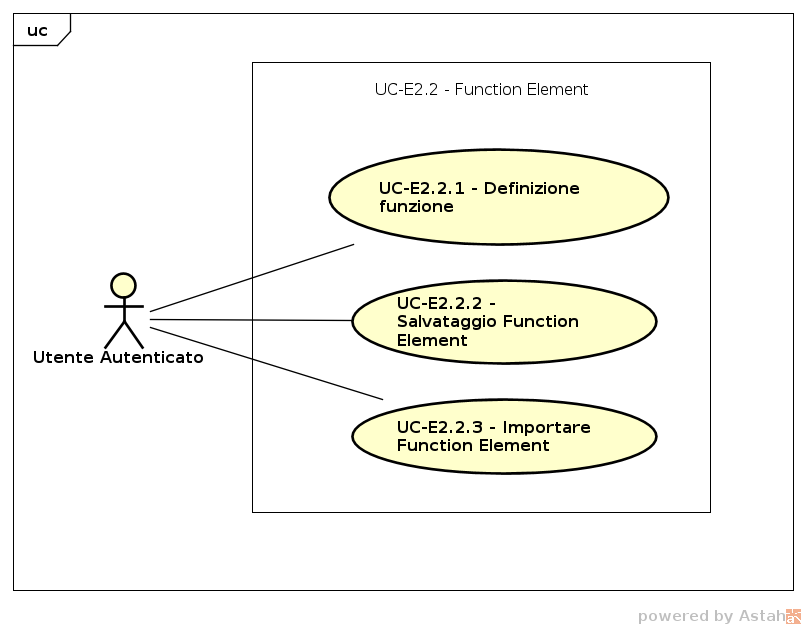
\includegraphics[width=12cm]{res/img/UCEditor/UC-E2.2-FunctionElement}
      \caption{UC-E2.2 - Function Element}
      \end{center} 
    \end{figure}

    %Tabella 
    \begin{center}
      \bgroup
      \def\arraystretch{1.8}     
      \begin{longtable}{  p{3.5cm} | p{8cm} } 
        
        \hline
        \multicolumn{2}{ | c | }{ \cellcolor[gray]{0.9} \textbf{UC-E2.2 - Function Element}} \\ 
        \hline
        
        \textbf{Attori Primari} & Utente Autenticato, Ospite, Membro, Admin, Proprietario \\ 
        \textbf{Scopo e Descrizione} & Rappresentare una canonica funzione in cui \`e possibile agganciare un elemento che verr\`a considerato un input e collegare l'output ad un altro DSL Element \\ 
        
        \textbf{Precondizioni}  & L'utente sta visualizzando l'editor \\ 
        
        \textbf{Postcondizioni} & L'utente ha collegato un function al valore del DSL desiderato \\ 
        \textbf{Flusso Principale} & 1. Definizione funzione (UC-E2.2.1)
2. Salvataggio Function Element (UC-E2.2.2)
3. Importare Function Element (UC-E2.2.3)  \\
        \textbf{Estensioni} &  \\
        \textbf{Inclusioni} & 
      \end{longtable}
      \egroup
    \end{center}
\subsubsection{UC-E2.2.1}

    %Tabella 
    \begin{center}
      \bgroup
      \def\arraystretch{1.8}     
      \begin{longtable}{  p{3.5cm} | p{8cm} } 
        
        \hline
        \multicolumn{2}{ | c | }{ \cellcolor[gray]{0.9} \textbf{UC-E2.2.1 - Definizione funzione}} \\ 
        \hline
        
        \textbf{Attori Primari} & Utente Autenticato, Ospite, Membro, Admin, Proprietario \\ 
        \textbf{Scopo e Descrizione} & L'utente ha la possibilit\`a di scrivere in un campo testo una funzione con il linguaggio definito da MaaS \\ 
        
        \textbf{Precondizioni}  & L'utente sta visualizzando l'editor \\ 
        
        \textbf{Postcondizioni} & L'utente ha definito con successo una funzione \\ 
        \textbf{Flusso Principale} &  \\
        \textbf{Estensioni} &  \\
        \textbf{Inclusioni} & 
      \end{longtable}
      \egroup
    \end{center}
\subsubsection{UC-E2.2.2}

    %Tabella 
    \begin{center}
      \bgroup
      \def\arraystretch{1.8}     
      \begin{longtable}{  p{3.5cm} | p{8cm} } 
        
        \hline
        \multicolumn{2}{ | c | }{ \cellcolor[gray]{0.9} \textbf{UC-E2.2.2 - Salvataggio Function Element}} \\ 
        \hline
        
        \textbf{Attori Primari} & Utente Autenticato, Ospite, Membro, Admin, Proprietario \\ 
        \textbf{Scopo e Descrizione} & L'utente ha la possibilit\`a di storicizzare la sua Function Element creata \\ 
        
        \textbf{Precondizioni}  & L'utente ha inserito una Function Element valida \\ 
        
        \textbf{Postcondizioni} & La Function Element \`e stata salvata con successo in MaaS \\ 
        \textbf{Flusso Principale} &  \\
        \textbf{Estensioni} &  \\
        \textbf{Inclusioni} & 
      \end{longtable}
      \egroup
    \end{center}
\subsubsection{UC-E2.2.3}

    %Tabella 
    \begin{center}
      \bgroup
      \def\arraystretch{1.8}     
      \begin{longtable}{  p{3.5cm} | p{8cm} } 
        
        \hline
        \multicolumn{2}{ | c | }{ \cellcolor[gray]{0.9} \textbf{UC-E2.2.3 - Importare Function Element}} \\ 
        \hline
        
        \textbf{Attori Primari} & Utente Autenticato, Ospite, Membro, Admin, Proprietario \\ 
        \textbf{Scopo e Descrizione} & Permette di importare nella sessione corrente una Function Element precedentemente definita \\ 
        
        \textbf{Precondizioni}  & L'utente ha i diritti per caricare la Function Element \\ 
        
        \textbf{Postcondizioni} & L'utente ha caricato la Function Element con successo \\ 
        \textbf{Flusso Principale} &  \\
        \textbf{Estensioni} &  \\
        \textbf{Inclusioni} & 
      \end{longtable}
      \egroup
    \end{center}
\subsubsection{UC-E2.3}
 

    \begin{figure}[H]
      \begin{center}
        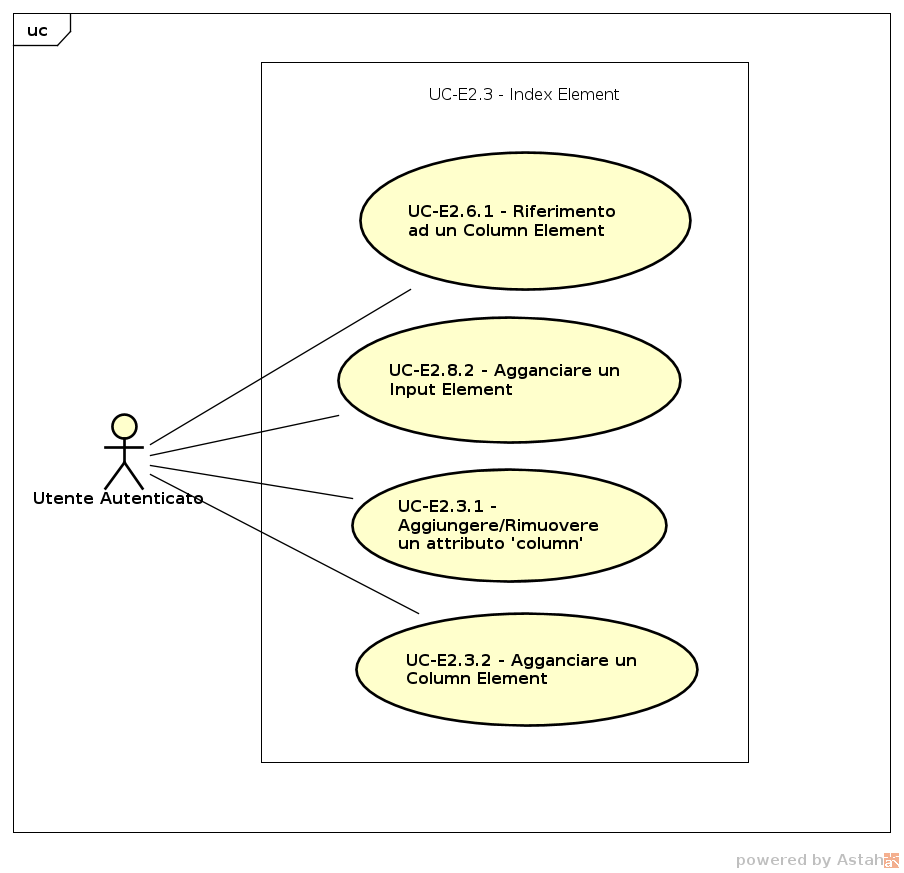
\includegraphics[width=12cm]{res/img/UCEditor/UC-E2.3-IndexElement}
      \caption{UC-E2.3 - Index Element}
      \end{center} 
    \end{figure}

    %Tabella 
    \begin{center}
      \bgroup
      \def\arraystretch{1.8}     
      \begin{longtable}{  p{3.5cm} | p{8cm} } 
        
        \hline
        \multicolumn{2}{ | c | }{ \cellcolor[gray]{0.9} \textbf{UC-E2.3 - Index Element}} \\ 
        \hline
        
        \textbf{Attori Primari} & Utente Autenticato, Ospite, Membro, Admin, Proprietario \\ 
        \textbf{Scopo e Descrizione} & Rappresentazione della sezione index del DSL nell'editor \\ 
        
        \textbf{Precondizioni}  & L'aggiunta dell'Index Element dev'essere eseguita in una Collection Element esistente \\ 
        
        \textbf{Postcondizioni} & \`E stata aggiunta la sezione Index alla Collection del DSL corrente \\ 
        \textbf{Flusso Principale} & 1. Riferimento ad un Column Element (UC-E2.6.1)
2. Agganciare un Input Element (UC-E2.8.2)
3. Aggiungere/Rimuovere un attributo ``column" (UC-E2.3.1)
4. Agganciare un Column Element (UC-E2.3.2) \\
        \textbf{Estensioni} &  \\
        \textbf{Inclusioni} & 
      \end{longtable}
      \egroup
    \end{center}
\subsubsection{UC-E2.3.1}

    %Tabella 
    \begin{center}
      \bgroup
      \def\arraystretch{1.8}     
      \begin{longtable}{  p{3.5cm} | p{8cm} } 
        
        \hline
        \multicolumn{2}{ | c | }{ \cellcolor[gray]{0.9} \textbf{UC-E2.3.1 - Aggiungere/Rimuovere un attributo ``column''}} \\ 
        \hline
        
        \textbf{Attori Primari} & Utente Autenticato, Ospite, Membro, Admin, Proprietario \\ 
        \textbf{Scopo e Descrizione} & Si da la possibilit\`a di rimuovere o aggiungere dall'Index un attributo \\ 
        
        \textbf{Precondizioni}  & Sia collegata a un Index Element \\ 
        
        \textbf{Postcondizioni} & Nel DSL nella sezione Index \`e aggiunto o rimosso un attributo ``column'' \\ 
        \textbf{Flusso Principale} &  \\
        \textbf{Estensioni} &  \\
        \textbf{Inclusioni} & 
      \end{longtable}
      \egroup
    \end{center}
\subsubsection{UC-E2.3.2}

    %Tabella 
    \begin{center}
      \bgroup
      \def\arraystretch{1.8}     
      \begin{longtable}{  p{3.5cm} | p{8cm} } 
        
        \hline
        \multicolumn{2}{ | c | }{ \cellcolor[gray]{0.9} \textbf{UC-E2.3.2 - Agganciare un Column Element}} \\ 
        \hline
        
        \textbf{Attori Primari} & Utente Autenticato, Ospite, Membro, Admin, Proprietario \\ 
        \textbf{Scopo e Descrizione} & \`E possibile agganciare un Column Element all'attributo ``column'' \\ 
        
        \textbf{Precondizioni}  & Deve essere presente un attributo Column \\ 
        
        \textbf{Postcondizioni} & La sezione del DSL ``column'' viene riempita con i valori impostati sul Column Element  \\ 
        \textbf{Flusso Principale} &  \\
        \textbf{Estensioni} &  \\
        \textbf{Inclusioni} & 
      \end{longtable}
      \egroup
    \end{center}
\subsubsection{UC-E2.4}

    %Tabella 
    \begin{center}
      \bgroup
      \def\arraystretch{1.8}     
      \begin{longtable}{  p{3.5cm} | p{8cm} } 
        
        \hline
        \multicolumn{2}{ | c | }{ \cellcolor[gray]{0.9} \textbf{UC-E2.4 - Column Element}} \\ 
        \hline
        
        \textbf{Attori Primari} & Utente Autenticato, Ospite, membro, Admin, Proprietario \\ 
        \textbf{Scopo e Descrizione} & Dare tutte le funzionalit\`a espresse nel DSL Element \\ 
        
        \textbf{Precondizioni}  & Deve riferirsi ad una struttura column presente nel DSL corrente \\ 
        
        \textbf{Postcondizioni} & L'utente manipola le parti che compongono la struttura \\ 
        \textbf{Flusso Principale} &  \\
        \textbf{Estensioni} &  \\
        \textbf{Inclusioni} & 
      \end{longtable}
      \egroup
    \end{center}
\subsubsection{UC-E2.5}

    %Tabella 
    \begin{center}
      \bgroup
      \def\arraystretch{1.8}     
      \begin{longtable}{  p{3.5cm} | p{8cm} } 
        
        \hline
        \multicolumn{2}{ | c | }{ \cellcolor[gray]{0.9} \textbf{UC-E2.5 - Row Element}} \\ 
        \hline
        
        \textbf{Attori Primari} & Utente Autenticato, Ospite, Membro, Admin, Proprietario \\ 
        \textbf{Scopo e Descrizione} & Rappresentazione di una struttura Row all'interno del DSL \\ 
        
        \textbf{Precondizioni}  & Dev'essere legata a una struttura Document \\ 
        
        \textbf{Postcondizioni} & Viene definita la struttura della Row all'interno del DSL corrente \\ 
        \textbf{Flusso Principale} &  \\
        \textbf{Estensioni} &  \\
        \textbf{Inclusioni} & 
      \end{longtable}
      \egroup
    \end{center}
\subsubsection{UC-E2.6}
 

    \begin{figure}[H]
      \begin{center}
        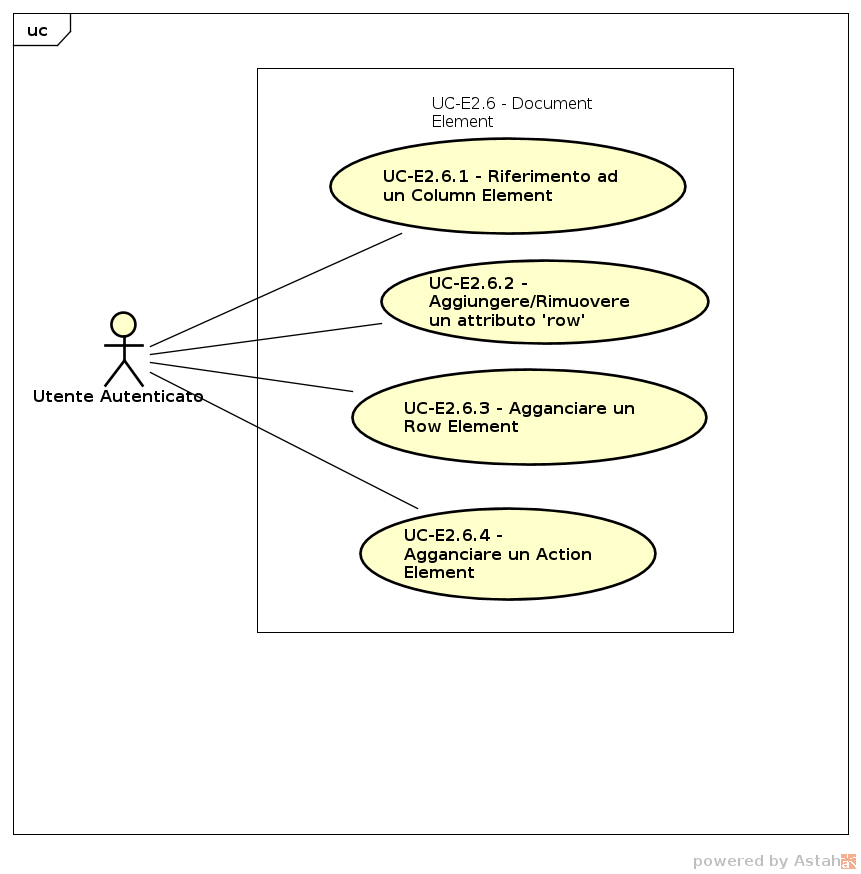
\includegraphics[width=12cm]{res/img/UCEditor/UC-E2.6-DocumentElement}
      \caption{UC-E2.6 - Document Element}
      \end{center} 
    \end{figure}

    %Tabella 
    \begin{center}
      \bgroup
      \def\arraystretch{1.8}     
      \begin{longtable}{  p{3.5cm} | p{8cm} } 
        
        \hline
        \multicolumn{2}{ | c | }{ \cellcolor[gray]{0.9} \textbf{UC-E2.6 - Document Element}} \\ 
        \hline
        
        \textbf{Attori Primari} & Utente Autenticato, Ospite, Membro, Admin, Proprietario \\ 
        \textbf{Scopo e Descrizione} & Rappresenta l'elemento Document del DSL \\ 
        
        \textbf{Precondizioni}  & L'utente visualizza l'editor \\ 
        
        \textbf{Postcondizioni} & Viene generato l'elemento Document nel DSL \\ 
        \textbf{Flusso Principale} & 1. Riferimento ad un Column Element (UC-E2.6.1)
2. Aggiungere/Rimuovere un attributo row (UC-E2.6.2)
3. Agganciare un Row Element (UC-E2.6.3)
4. Agganciare un Action Element (UC-E2.6.4) \\
        \textbf{Estensioni} &  \\
        \textbf{Inclusioni} & 
      \end{longtable}
      \egroup
    \end{center}
\subsubsection{UC-E2.6.1}

    %Tabella 
    \begin{center}
      \bgroup
      \def\arraystretch{1.8}     
      \begin{longtable}{  p{3.5cm} | p{8cm} } 
        
        \hline
        \multicolumn{2}{ | c | }{ \cellcolor[gray]{0.9} \textbf{UC-E2.6.1 - Riferimento ad un Column Element}} \\ 
        \hline
        
        \textbf{Attori Primari} & Utente Autenticato, Ospite, Membro, Admin, Proprietario \\ 
        \textbf{Scopo e Descrizione} & Riferirsi ad un elemento colonna precedentemente definito in modo da applicare la populate del DSL \\ 
        
        \textbf{Precondizioni}  & Esista almeno un elemento Document a cui si riferisca \\ 
        
        \textbf{Postcondizioni} & Viene composta la funzione populate \\ 
        \textbf{Flusso Principale} &  \\
        \textbf{Estensioni} &  \\
        \textbf{Inclusioni} & 
      \end{longtable}
      \egroup
    \end{center}
\subsubsection{UC-E2.6.2}

    %Tabella 
    \begin{center}
      \bgroup
      \def\arraystretch{1.8}     
      \begin{longtable}{  p{3.5cm} | p{8cm} } 
        
        \hline
        \multicolumn{2}{ | c | }{ \cellcolor[gray]{0.9} \textbf{UC-E2.6.2 - Aggiungere/Rimuovere un attributo row}} \\ 
        \hline
        
        \textbf{Attori Primari} & Utente Autenticato, Ospite, Membro, Admin, Proprietario \\ 
        \textbf{Scopo e Descrizione} & Aggiungere o rimuovere una struttura ``row'' all'interno del Document nella struttura DSL \\ 
        
        \textbf{Precondizioni}  & Si deve riferire a un Document esistente \\ 
        
        \textbf{Postcondizioni} & \`E stata manipolata (aggiunta o rimossa) una ``row'' all'interno del DSL Document \\ 
        \textbf{Flusso Principale} &  \\
        \textbf{Estensioni} &  \\
        \textbf{Inclusioni} & 
      \end{longtable}
      \egroup
    \end{center}
\subsubsection{UC-E2.6.3}

    %Tabella 
    \begin{center}
      \bgroup
      \def\arraystretch{1.8}     
      \begin{longtable}{  p{3.5cm} | p{8cm} } 
        
        \hline
        \multicolumn{2}{ | c | }{ \cellcolor[gray]{0.9} \textbf{UC-E2.6.3 - Agganciare un Row Element}} \\ 
        \hline
        
        \textbf{Attori Primari} & Utente Autenticato, Ospite, Membro, Admin, Proprietario \\ 
        \textbf{Scopo e Descrizione} & Definire la struttura della ``row'' del DSL  \\ 
        
        \textbf{Precondizioni}  & Sia presente un attributo ``row'' nel Document \\ 
        
        \textbf{Postcondizioni} & Nel DSL vengono trascritti nella struttura ``row'' gli attributi e i rispettivi valori \\ 
        \textbf{Flusso Principale} &  \\
        \textbf{Estensioni} &  \\
        \textbf{Inclusioni} & 
      \end{longtable}
      \egroup
    \end{center}
\subsubsection{UC-E2.6.4}

    %Tabella 
    \begin{center}
      \bgroup
      \def\arraystretch{1.8}     
      \begin{longtable}{  p{3.5cm} | p{8cm} } 
        
        \hline
        \multicolumn{2}{ | c | }{ \cellcolor[gray]{0.9} \textbf{UC-E2.6.4 - Agganciare un Action Element}} \\ 
        \hline
        
        \textbf{Attori Primari} & Utente Autenticato, Ospite, Membro, Admin, Proprietario \\ 
        \textbf{Scopo e Descrizione} & Legare il contenuto informativo della ``row'' all'azione definita dalla ``action'' \\ 
        
        \textbf{Precondizioni}  & \`E definita una ``row'' all'interno del DSL \\ 
        
        \textbf{Postcondizioni} & Verr\`a definita la ``action'' nella ``row'' \\ 
        \textbf{Flusso Principale} &  \\
        \textbf{Estensioni} &  \\
        \textbf{Inclusioni} & 
      \end{longtable}
      \egroup
    \end{center}
\subsubsection{UC-E2.7}
 

    \begin{figure}[H]
      \begin{center}
        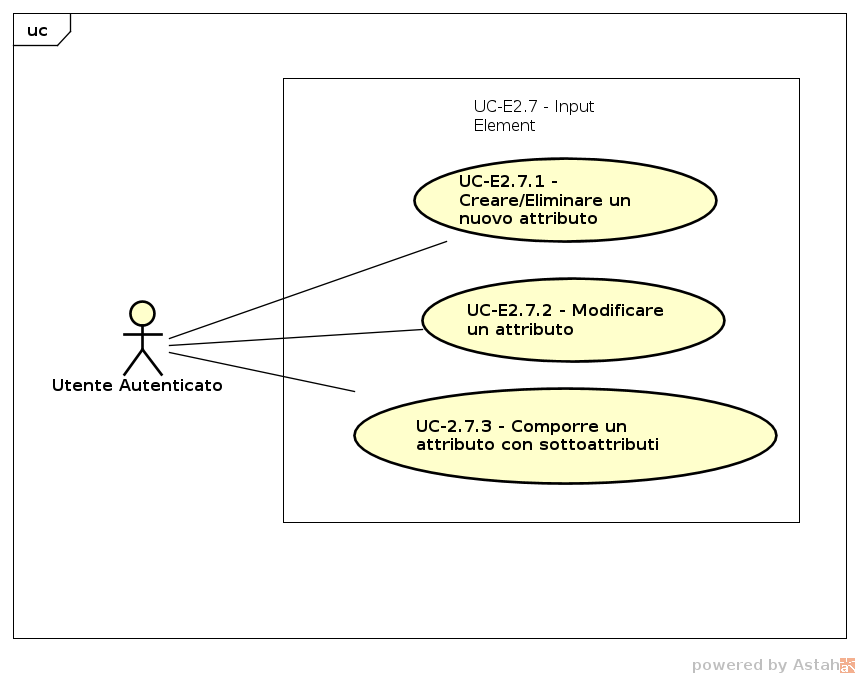
\includegraphics[width=12cm]{res/img/UCEditor/UC-E2.7-InputElement}
      \caption{UC-E2.7 - Input Element}
      \end{center} 
    \end{figure}

    %Tabella 
    \begin{center}
      \bgroup
      \def\arraystretch{1.8}     
      \begin{longtable}{  p{3.5cm} | p{8cm} } 
        
        \hline
        \multicolumn{2}{ | c | }{ \cellcolor[gray]{0.9} \textbf{UC-E2.7 - Input Element}} \\ 
        \hline
        
        \textbf{Attori Primari} & Utente Autenticato, Ospite, Membro, Admin, Proprietario \\ 
        \textbf{Scopo e Descrizione} & Si occupa di rappresentare una dato in un specifico formato \\ 
        
        \textbf{Precondizioni}  & L'utente pu\`o visualizzare l'Editor \\ 
        
        \textbf{Postcondizioni} & Viene composto il dato con i valori inseriti dall'utente \\ 
        \textbf{Flusso Principale} & 1. Creare/Eliminare un nuovo attributo (UC-E2.7.1)
2. Modificare un attributo (UC-E2.7.2)
3. Comporre un attributo con sottoattributi (UC-E2.7.3) \\
        \textbf{Estensioni} &  \\
        \textbf{Inclusioni} & 
      \end{longtable}
      \egroup
    \end{center}
\subsubsection{UC-E2.7.1}

    %Tabella 
    \begin{center}
      \bgroup
      \def\arraystretch{1.8}     
      \begin{longtable}{  p{3.5cm} | p{8cm} } 
        
        \hline
        \multicolumn{2}{ | c | }{ \cellcolor[gray]{0.9} \textbf{UC-E2.7.1 - Creare/Eliminare un nuovo attributo}} \\ 
        \hline
        
        \textbf{Attori Primari} & Utente Autenticato, Ospite, Membro, Admin, Proprietario \\ 
        \textbf{Scopo e Descrizione} & Essendo il dato componibile da pi\`u attributi, permette di definire una coppia chiave/valore per meglio definire il suo dato \\ 
        
        \textbf{Precondizioni}  & L'utente si deve riferire a un Data Element presente \\ 
        
        \textbf{Postcondizioni} & Si manipola l'attributo selezionato \\ 
        \textbf{Flusso Principale} &  \\
        \textbf{Estensioni} &  \\
        \textbf{Inclusioni} & 
      \end{longtable}
      \egroup
    \end{center}
\subsubsection{UC-E2.7.2}

    %Tabella 
    \begin{center}
      \bgroup
      \def\arraystretch{1.8}     
      \begin{longtable}{  p{3.5cm} | p{8cm} } 
        
        \hline
        \multicolumn{2}{ | c | }{ \cellcolor[gray]{0.9} \textbf{UC-E2.7.2 - Modificare un attributo}} \\ 
        \hline
        
        \textbf{Attori Primari} & Utente Autenticato, Ospite, Membro, Admin, Proprietario \\ 
        \textbf{Scopo e Descrizione} & Poter rinominare o la chiave o il valore all'interno di un Data Element \\ 
        
        \textbf{Precondizioni}  & Ci sia un attributo a cui riferirsi \\ 
        
        \textbf{Postcondizioni} & Viene modificata o la chiave o il valore dell'attributo selezionato dall'utente \\ 
        \textbf{Flusso Principale} &  \\
        \textbf{Estensioni} &  \\
        \textbf{Inclusioni} & 
      \end{longtable}
      \egroup
    \end{center}
\subsubsection{UC-E2.7.3}

    %Tabella 
    \begin{center}
      \bgroup
      \def\arraystretch{1.8}     
      \begin{longtable}{  p{3.5cm} | p{8cm} } 
        
        \hline
        \multicolumn{2}{ | c | }{ \cellcolor[gray]{0.9} \textbf{UC-E2.7.3 - Comporre un attributo con sottoattributi}} \\ 
        \hline
        
        \textbf{Attori Primari} & Utente Autenticato, Ospite, Membro, Admin, Proprietario \\ 
        \textbf{Scopo e Descrizione} & Un utente \`e in grado di poter definire strutture complesse per i suoi scopi \\ 
        
        \textbf{Precondizioni}  & Ci sia un Data Element a cui riferirsi \\ 
        
        \textbf{Postcondizioni} & L'attributo del dato \`e a sua volta costituito da altri attributi \\ 
        \textbf{Flusso Principale} &  \\
        \textbf{Estensioni} &  \\
        \textbf{Inclusioni} & 
      \end{longtable}
      \egroup
    \end{center}

\section{Interprete}
\subsection{Diagrammi della classi}
L'interprete è la componente di MaaS che si occupa della conversione da DSL Structure in DSL. Questa decisione è stata presa per poter avere una rappresentazione semplice da manipolare attraverso l'editor e facile da ricondurre nel formato testuale.

La progettazione ha seguito un approccio bottom-up, con la creazione delle componenti per il funzionamento, incluse in un package e inserito un Facade per semplificarne l'uso. I patter usati sono Facade, Singleton e Chain of Responsability.
\subsection{Package DSLInterpreter}
\begin{figure}[H]
  \centering
  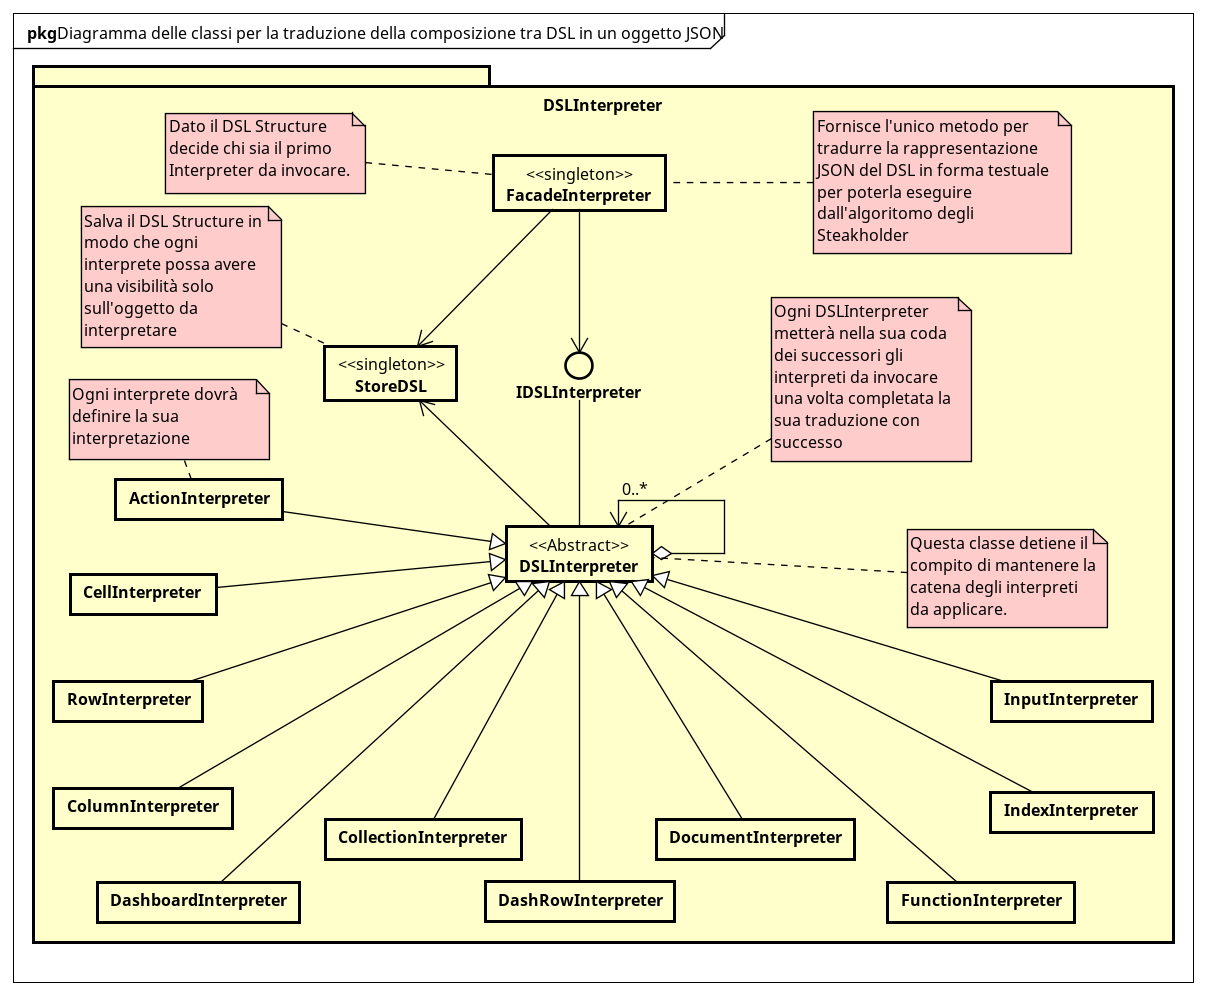
\includegraphics[width=0.9\textwidth]{res/img/Diagram_Interpreter.png}
  \caption{Package DSLInterpreter}
  \label{fig:diagram_model}
\end{figure}
\subsubsection{Descrizione}
In questo package vengono inserite tutte le classi che contribuiscono alla traduzione dal DSL Structure prodotto dall'editor all'equivalente DSL.
La classe DSLInterpreter implementa il Chain of Responsability dove detiene una lista di tutti gli interpreti da invocare man mano che vengono applicate le traduzioni. Il risultato di ogni interprete verrà contatenato e come risultato si otterrà il DSL richiesto.
Il FacadeEditorInterpreter implementa il patter Facade per offrire un interfaccia semplice per attuare la traduzione rendendo nascoste i componenti per applicarla.
\subsubsection{DSLInterpreter::FacadeInterpreter}
\begin{itemize}
\item \textbf{Descrizione} \hfill \\
  Rappresenta l'implementazione del pattern Facade.
\item \textbf{Utilizzo} \hfill \\
  Permette di interfacciarsi al modulo richiedendo eslusivamente la traduzione da DSL Structure a DSL. Questo oltre a semplificare al client la gestione della traduzione, nasconde l'implementazione rendendo il modulo maggiormente mantenibile.
\item \textbf{Relazioni con altre classi} \hfill
  \begin{itemize}
  \item DSLInterpreter::StoreDSL
  \item DSLInterpreter::IDSLInterpreter
  \end{itemize}
\end{itemize}
\subsubsection{DSLInterpreter::StoreDSL}
\begin{itemize}
\item \textbf{Descrizione} \hfill \\
  Mantiene il riferimento dal DSL Structure da tradurre.
\item \textbf{Utilizzo} \hfill \\
  Viene usata dalle implementazioni di \texttt{DSLInterpreter::DSLInterpreter} per ottenere l'oggetto riferito da un attributo della struttura da tradurre. Questi casi si riscontrano nella definizione di un componente del DSL in cui sono innestati altri componenti ( es. DSL Collection con DSL Index e DSL Document ).

  Ciò permette di non violare il Single Responsability Principle, in quanto i vari interpreti conoscono solo la struttura del singolo componente da interpretare e non detengono un possibile accesso dell'intera DSL Structure.
\item \textbf{Relazione con altre classi} \hfill
  \begin{itemize}
  \item DSLInterpreter::DSLFacadeInterpreter
  \item DSLInterpreter::DSLInterpreter
  \end{itemize}
\end{itemize}
\subsubsection{DSLInterpreter::DSLInterpreter}
\begin{itemize}
\item \textbf{Descrizione}
  Implementa il Chain of Responsabiltity mantenendo una lista di tutti gli interpreti da avviare e fornisce i metodo da implementare per i vari interpreti.
\item \textbf{Utilizzo}
  Mantiene struttura dati ed il comportamento comune degli interpreti. In più attraverso il metodo interpret viene definita la sequenza per portare a compito la traduzione di una componente del DSL.
\item \textbf{Relazione con altre classi} \hfill
  \begin{itemize}
  \item DSLInterpreter::FacadeInterpreter
  \item DSLInterpreter::StoreDSL
  \item DSLInterpreter::ActionInterpreter
  \item DSLInterpreter::CellInterpreter
  \item DSLInterpreter::RowInterpreter
  \item DSLInterpreter::ColumnInterpreter
  \item DSLInterpreter::DashboardInterpreter
  \item DSLInterpreter::CollectionInterpreter
  \item DSLInterpreter::DashRowInterpreter
  \item DSLInterpreter::DocumentInterpreter
  \item DSLInterpreter::FunctionInterpreter
  \item DSLInterpreter::IndexInterpreter
  \item DSLInterpreter::InputInterpreter
  \end{itemize}
\end{itemize}

 
\section{Frontend}

\subsection{Descrizione generale}

Il frontend dell'applicazione andrà a costituire il ruolo di \textit{View} nel pattern MVC. In particolare tale componente dell'applicazione è costituita da un sottosistema che implementa l'architettura \textit{Flux} proposta da \textit{Facebook}. Tale architettura si basa sul creare un sistema che abbia un \textit{data-flow} unidirezionale al fine di semplificare le interazioni tra le varie componenti e di assicurare che tra le componenti non esistano dipendenze circolari.
Nella progettazione secondo l'architettura \textit{Flux} si è seguito in particolare il principio che nessuna classe modifichi direttamente lo stato di un'altra ma che vengano create delle componenti che richiedono un'interazione delle \textit{Action} per comunicare con le altre parti del sistema.

\begin{figure}[h]
\centering
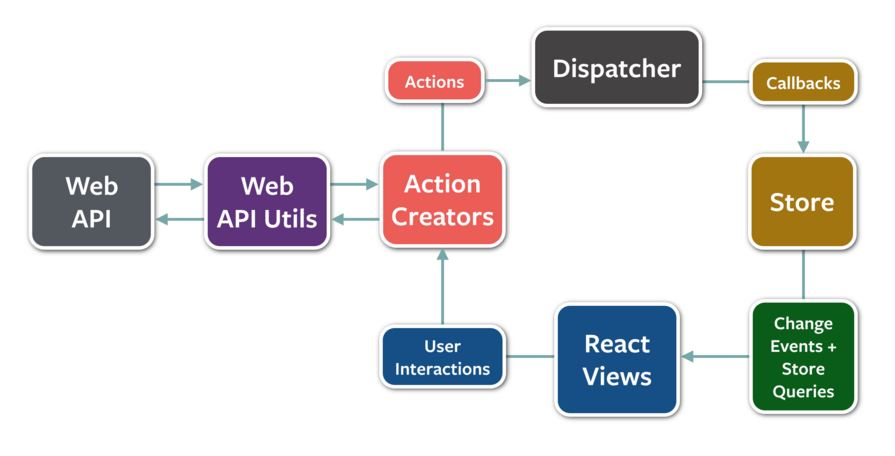
\includegraphics[width=0.8\textwidth]{res/sections/imgs/flux.jpg}
\caption{Diagramma dell'architettura Flux di Facebook}
\end{figure}
In un'architettura \textit{Flux} vengono distinti 4 componenti fondamentali:

\begin{itemize}
\item \textbf{Action}: Rappresenta un messaggio tra le componenti del sistema;
\item \textbf{Dispatcher}: funge da \textit{hub} centrale per le \textit{action} e si occupa di distribuirle al giusto \textit{store};
\item \textbf{Store}: contengono la logica applicativa del frontend e lo stato dei dati dall'ultimo \textit{update}. Si occupano di fornire i dati alle viste, quando queste li richiedono;
\item \textbf{View}: Sono la parte visiva dell'applicazione e, nel nostro caso, saranno costituite da componenti definite con React.
\end{itemize}

Dall'architettura sopra descritta sono stati individuati i seguenti package per il lato frontend di MaaS:

\begin{figure}[h]
\centering
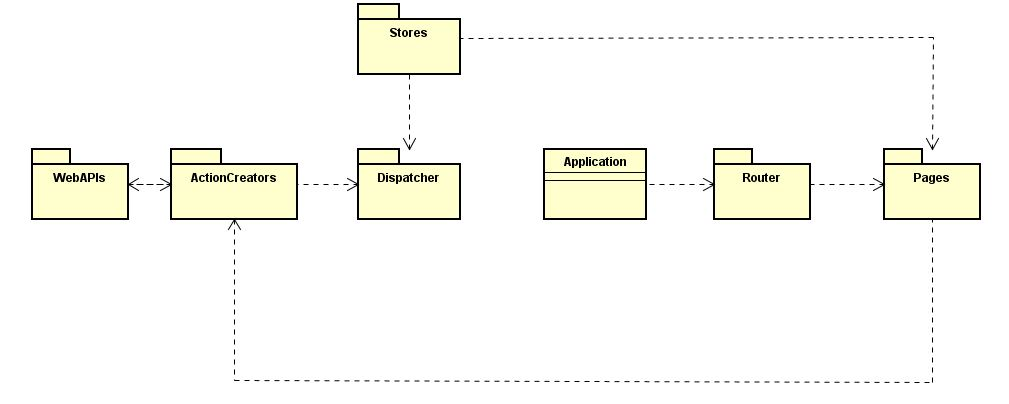
\includegraphics[width=0.8\textwidth]{res/sections/imgs/packages-diagram.jpg}
\caption{Diagramma dei package del frontend}
\end{figure}

\section{Descrizione dei package del frontend}
\subsection{WebAPIs}

\begin{figure}[h]
\centering
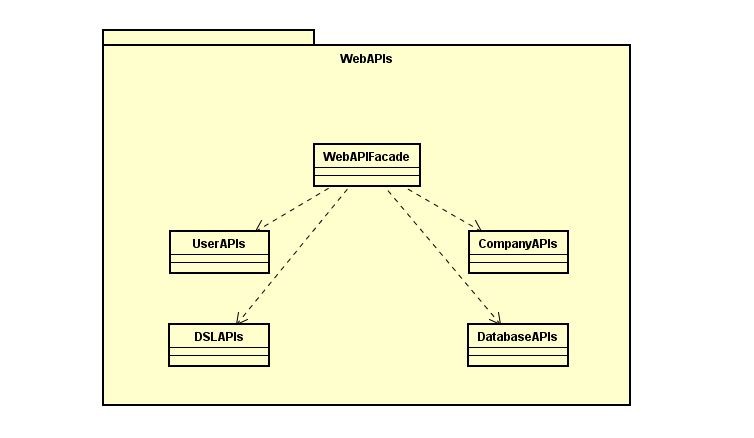
\includegraphics[width=0.8\textwidth]{res/sections/imgs/webapi-diagram.jpg}
\caption{Diagramma dei package del frontend}
\end{figure}

\paragraph*{Descrizione del package}
Il seguente package contiene tutte le classi che contengono i metodi per interagire con le API esposte dal server. 
\paragraph*{Classi contenute}
\begin{itemize}
\item \textbf{UserAPIs};
\item \textbf{CompanyAPIs};
\item \textbf{DSLAPIs};
\item \textbf{DatabaseAPIs};
\item \textbf{WebAPIFacade}.
\end{itemize}

\subsubsection{UserAPIs}
\paragraph*{Descrizione della classe}
Classe che espone tutti i metodi per interagire con le API del server che riguardano gli utenti.

\paragraph*{Utilizzo}
Viene utilizzata sia per il login sia per gestire le operazioni CRUD per le informazioni riguardanti gli utenti.

\paragraph*{Relazione con altre classi}
\begin{itemize}
\item ActionCreators::UserActionCreator
\end{itemize}

\subsubsection{CompanyAPIs}
\paragraph*{Descrizione della classe}
Classe che espone i metodi per interagire con le API esposte dal server che riguardano le Company.

\paragraph*{Utilizzo}
Contiene le operazioni CRUD per interagire con le informazioni riguardanti le company utilizzando le API esposte dal backend.

\paragraph*{Relazione con altre classi}
\begin{itemize}
\item ActionCreators::CompanyActionCreator
\end{itemize}

\subsubsection{DSLAPIs}
\paragraph*{Descrizione della classe}
Classe che espone i metodi per interagire con le API esposte dal server che riguardano le specifiche DSL.

\paragraph*{Utilizzo}
Viene utilizzata per lanciare le operazioni CRUD associate alle API esposte dal backend.

\paragraph*{Relazione con altre classi}
\begin{itemize}
\item ActionCreators::DSLActionCreator
\end{itemize}

\subsubsection{DatabaseAPIs}
\paragraph*{Descrizione della classe}
Classe per interagire con le API esposte dal server che riguardano i database delle Company.

\paragraph*{Utilizzo}
Viene utilizzata questa classe per lanciare le operazioni CRUD esposte dalle API del backend.

\paragraph*{Relazione con altre classi}
\begin{itemize}
\item ActionCreators::DatabaseAPIs
\end{itemize}

\subsubsection{WebAPIFacade}
\paragraph*{Descrizione della classe}
Classe che implementa il \textit{design pattern} \textit{Facade} al fine di creare un'interfaccia semplificata per il resto delle componenti per interagire con le API esposte dal backend.
\paragraph*{Utilizzo}
Questa classe viene utilizzata come interfaccia per il frontend per comunicare con le API esposte dal backend.
\paragraph*{Relazione con altre classi}
\begin{itemize}
\item webAPIs;
\item actionCreators.
\end{itemize} 

\subsection{ActionCreators}

\begin{figure}[h]
\centering
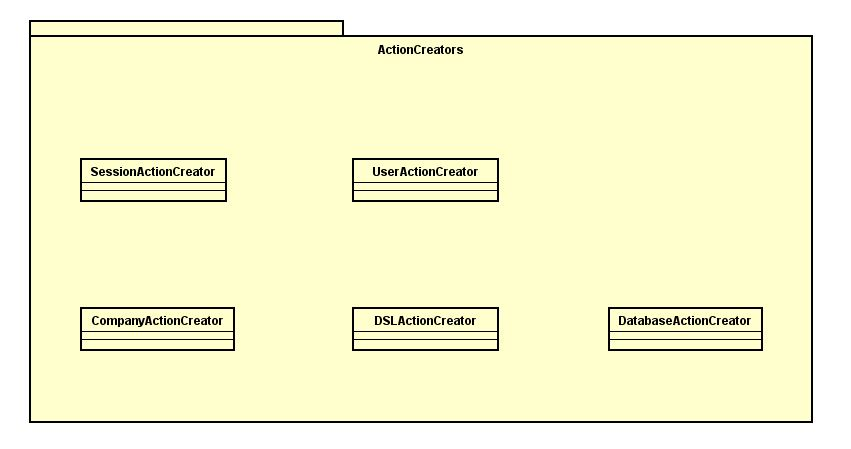
\includegraphics[width=0.8\textwidth]{res/sections/imgs/actioncreator-diagram.jpg}
\caption{Diagramma delle classi contenute in ActionCreators}
\end{figure}

\paragraph*{Descrizione del package}
Questo package contiene tutte le classi che si prestano come factory di Action. Le classi in questione mettono in relazione le webAPIs con il resto dell'applicazione, cioè vengono utilizzate per la richiesta delle funzionalità delle webAPIs per poi lanciare le Action relative alle risposte ricevute.

\paragraph*{Classi contenute}
\begin{itemize}
\item \textbf{SessionActionCreator};
\item \textbf{UserActionCreator};
\item \textbf{CompanyActionCreator};
\item \textbf{DSLActionCreator};
\item \textbf{DatabaseActionCreator}.
\end{itemize}

\subsubsection{SessionActionCreator}
\paragraph*{Descrizione della classe}
Classe che si occupa della gestione delle \textit{action} relative alla sessione corrente.

\paragraph*{Utilizzo}
Viene utilizzata per richiedere il login di un utente e per emanare le \textit{action} relative a login, sessione corrente e logout.

\paragraph*{Relazione con altre classi}
\begin{itemize}
\item Dispatcher;
\item Pages;
\item webAPIs::WebAPIFacade;
\item Stores::SessionStore.
\end{itemize}

\subsubsection{UserActionCreator}
\paragraph*{Descrizione della classe}
Classe che si occupa di creare e lanciare le \textit{action} relative agli utenti. Viene implementata tramite il \textit{design pattern} \textit{Factory}.
\paragraph*{Utilizzo}
Viene utilizzata per creare le \textit{action} relative agli utenti: la classe fornisce i metodi per utilizzare le \textit{webAPIs} contenute relative all'utente e restituisce le action che poi verrano reindirizzate a UserStore.

\paragraph*{Relazione con altre classi}
\begin{itemize}
\item Dispatcher;
\item Pages;
\item webAPIs::WebAPIFacade;
\item Stores::UserStore.
\end{itemize}

\subsubsection{CompanyActionCreator}
\paragraph*{Descrizione della classe}
Classe che si occupa dell'interazione dell'applicazione con CompanyAPIs e di lanciare \textit{Action} relative alle risposte ottenute da essa. Viene implementata tramite \textit{design pattern} \textit{Factory}.
\paragraph*{Utilizzo}
La classe viene utilizzata per creare le \textit{action} relative alle Company: sfrutta le \textit{webAPIs} dichiarate per interagire con il server e lancia le \textit{action} contenenti i dati ricevuti dalle API richieste.

\paragraph*{Relazione con altre classi}
\begin{itemize}
\item Dispatcher;
\item Pages;
\item Stores::CompanyStore;
\item webAPIs::WebAPIFacade.
\end{itemize}

\subsubsection{DSLActionCreator}
\paragraph*{Descrizione della classe}
Classe che si occupa di creare \textit{action} riguardanti le specifiche DSL.
\paragraph*{Utilizzo}
Tale classe viene utilizzata per sfruttare i metodi dichiarati dalle webAPIs per la richiesta delle API esposte dal server relative alle specifiche DSL. Dopo aver sfruttato l'API richiesta, la classe crea un'\textit{action} contenente i risultati ottenuti.

\paragraph*{Relazione con altre classi}
\begin{itemize}
\item Dispatcher;
\item Stores::DSLStore;
\item Pages;
\item webAPIs::WebAPIFacade.
\end{itemize}

\subsubsection{DatabaseActionCreator}
\paragraph*{Descrizione della classe}
Classe che si occupa di lanciare \textit{action} riguardanti le connessioni ai database di una Company.
\paragraph*{Utilizzo}
La classe viene utilizzata per richiamare i metodi definiti dalle \textit{webAPIs} relativi ai database delle Company e creare le action contenenti le risposte dai metodi chiamati.
\paragraph*{Relazione con altre classi}
\begin{itemize}
\item Dispatcher;
\item Pages;
\item Store::DatabaseStore;
\item webAPIs::WebAPIFacade.
\end{itemize}

\subsection{Dispatcher}
\paragraph*{Descrizione della classe}
Classe raffigurante il \textit{dispatcher} descritto nell'architettura Flux.
\paragraph*{Utilizzo}
Il dispatcher viene utilizzato come \textit{hub} centrale delle \textit{action} circolanti per l'applicazione. Esso deve fornire le informazioni per instradare le \textit{action} create dagli ActionCreators verso il giusto Store di destinazione
\paragraph*{Relazione con altre classi}
\begin{itemize}
\item Stores;
\item ActionCreators.
\end{itemize}


\subsection{Stores}

\begin{figure}[h]
\centering
\includegraphics[width=0.8\textwidth]{res/sections/imgs/stores-diagram.jpg}
\caption{Diagramma delle classi per il package Stores}
\end{figure}

\paragraph*{Descrizione del package}
Il package in questione contiene le classi che implementano il concetto di Store presentato nell'architettura Flux. Ciascuno Store contiene dei dati omogenei tra loro e si occupa di fornirli alle pagine che ne necessitano.
\paragraph*{Classi contenute}
\begin{itemize}
\item \textbf{SessionStore};
\item \textbf{UserStore};
\item \textbf{DatabaseStore};
\item \textbf{CompanyStore};
\item \textbf{DSLStore}.
\end{itemize}

\subsubsection{SessionStore}
\paragraph*{Descrizione della classe}
Classe che contiene i dati relativi alla sessione corrente.
\paragraph*{Utilizzo}
Classe che viene utilizzata dall'applicazione per contenere e fornire i dati relativi alla sessione corrente. Si occupa di gestire le \textit{action} relative alla sessione e di conservarne i dati.
\paragraph*{Relazione con altre classi}
\begin{itemize}
\item Router;
\item Pages.
\end{itemize}

\subsubsection{UserStore}
\paragraph*{Descrizione della classe}
Classe che si occupa di contenere i dati relativi agli User.
\paragraph*{Utilizzo}
Questa classe viene utilizzata per mantenere i dati riguardanti gli utenti e di fornirli alle pagine che li richiedono.
\paragraph*{Relazione con altre classi}
\begin{itemize}
\item Pages;
\item Dispatcher.
\end{itemize}

\subsubsection{DatabaseStore}
\paragraph*{Descrizione della classe}
Classe che si occupa di contenere i dati relativi alle connessioni ai database definiti per le Company.
\paragraph*{Utilizzo}
Questa classe viene utilizzata per contenere i dati riguardanti le connessioni dei database definiti per le Company. Si occupa di ricevere dal dispatcher le \textit{action} relative a questi dati e di mantenere i dati riferiti.
\paragraph*{Relazione con altre classi}
\begin{itemize}
\item Pages;
\item Dispatcher.
\end{itemize}

\subsubsection{CompanyStore}
\paragraph*{Descrizione della classe}
Classe che si occupa di contenere i dati relativi alle Company.
\paragraph*{Utilizzo}
Questa classe viene utilizzata per ricevere le \textit{action} relative alle Company al fine di mantenere i dati relativi ad esse. Inoltre fornisce i metodi per fornire tali dati alle pagine che li richiedono
\paragraph*{Relazione con altre classi}
\begin{itemize}
\item Dispatcher;
\item Pages.
\end{itemize}

\subsubsection{DSLStore}
\paragraph*{Descrizione della classe}
Classe che si occupa di contenere i dati delle specifiche DSL
\paragraph*{Utilizzo}
Questa classe fornisce i metodi per ricevere le Action relative alle specifiche DSL e per mantenere i dati relativi ad esse. Fornisce inoltre i metodi per disporre quei dati per le pagine che li richiedono.
\paragraph*{Relazione con altre classi}
\begin{itemize}
\item Dispatcher;
\item Pages.
\end{itemize}


\subsection{Application}
\paragraph*{Descrizione della classe}
Questa è la classe principale del frontend: è la classe che richiama il Router e che inizializza il frontend.
\paragraph*{Utilizzo}
Viene utilizzata per inizializzare il frontend e per fornire le configurazioni necessarie al funzionamento per l'applicazione.

\subsection{Router}
\paragraph*{Descrizione della classe}
Questa classe è necessaria all'applicazione per determinare quale pagina mostrare.
\paragraph*{Utilizzo}
Viene istanziata nell'applicazione principale e determina le associazioni tra pagine e gli indirizzi URL per identificarle.

\subsection{Pages}
\paragraph*{Descrizione del package}
Questo package contiene tutte le pagine richiamate da Router. Ciascuna classe rappresenta una pagina definita come componente React e fornisce i metodi alla pagina per recuperare i dati da mostrare dagli store e i metodi per richiamare gli ActionCreators per la creazione di nuove Action.

    \end{tabular}
  \end{table}
  
\end{center}
